% !TeX document-id = {b657b89f-3a7b-42a1-879d-53584fcd9464}
% !TeX spellcheck = en_GB
% !TeX TS-program = lualatex

\documentclass[final,aspectratio=169,12pt]{beamer}

\usepackage[english]{babel}

%\usetheme{plain}
%\usepackage[math-style=ISO,warnings-off={mathtools-colon,mathtools-overbracket}]{unicode-math}
%\usepackage{lualatex-math}
\usepackage[no-math]{fontspec}
\usepackage[defaultmathsizes, basic]{mathastext}
\usepackage{fontawesome5}
%\setmathfont{Latin Modern Math}
%\setmathfont{Source Sans Pro}
\setmonofont{Inconsolata SemiBold}
%\setmathfont[range=\symup]{Latin Modern Roman}
\DeclareMathAlphabet{\Lmathit}{\encodingdefault}{\familydefault}{m}{it}

\setmainfont{SourceSansPro}

\newfontfamily{\titlefont}{League Gothic Regular}[]
\usepackage{amsmath}
\usepackage{xcolor}
\usepackage{tikz}
\usetikzlibrary{matrix,positioning,calc,fit,shapes,scopes,arrows.meta,backgrounds,decorations.markings,3d,decorations.pathreplacing,node-families,overlay-beamer-styles}

% also works for colorblind
\definecolor{SeqGrey1}{HTML}{595959}
\definecolor{SeqGrey2}{HTML}{808080}
\definecolor{SeqGrey3}{HTML}{B1B1B1}
\definecolor{SeqGrey4}{HTML}{ECECEC}

\definecolor{SeqGreen1}{HTML}{003213}
\definecolor{SeqGreen2}{HTML}{277D35}
\definecolor{SeqGreen3}{HTML}{6AB969}
\definecolor{SeqGreen4}{HTML}{B6E6AE}

\definecolor{SeqBlue1}{HTML}{124066}
\definecolor{SeqBlue2}{HTML}{2279BF}
\definecolor{SeqBlue3}{HTML}{2EA1FF}
\definecolor{SeqBlue4}{HTML}{A7C7FD}

\definecolor{SeqYellow1}{HTML}{735805}
\definecolor{SeqYellow2}{HTML}{d1a009}
\definecolor{SeqYellow3}{HTML}{F7CB45}
\definecolor{SeqYellow4}{HTML}{fdf0c9}

\definecolor{SeqRed1}{HTML}{7c0307}
\definecolor{SeqRed2}{HTML}{DC050C}
\definecolor{SeqRed3}{HTML}{fb5b61}
\definecolor{SeqRed4}{HTML}{fdbbbd}

\definecolor{BuRdBlue1}{HTML}{2166AC}
\definecolor{BuRdBlue2}{HTML}{4393C3}
\definecolor{BuRdBlue3}{HTML}{92C5DE}
\definecolor{BuRdBlue4}{HTML}{D1E5F0}
\definecolor{BuRdMidpoint}{HTML}{F7F7F7}
\definecolor{BuRdRed4}{HTML}{FDDBC7}
\definecolor{BuRdRed3}{HTML}{F4A582}
\definecolor{BuRdRed2}{HTML}{D6604D}
\definecolor{BuRdRed1}{HTML}{B2182B}
\definecolor{BuRdBadData}{HTML}{FFEE99}

\definecolor{BgColor}{HTML}{f5f5f5}

\setbeamerfont{frametitle}{size=\Huge,family=\titlefont}
\setbeamerfont{title}{size=\Huge,family=\titlefont}
\beamertemplatenavigationsymbolsempty
%\setbeamertemplate{footline}[page number]
%\addtobeamertemplate{navigation symbols}{}{%
%    \usebeamerfont{footline}%
%    \usebeamercolor[fg]{footline}%
%    %\hspace{1em}%
%    \normalsize\insertframenumber
%}

% access relative slide number (animations)
\makeatletter
\def\c@slideinframe{\beamer@slideinframe}
\def\beamerslideinframe{\beamer@slideinframe}
\makeatother

\setbeamertemplate{footline}{
  \hfill%
  \usebeamercolor[fg]{page number in head/foot}%
  \usebeamerfont{page number in head/foot}%
  \setbeamertemplate{page number in head/foot}[framenumber]%
  %\usebeamertemplate*{page number in head/foot}\alph{slideinframe}\kern1em\vskip2pt%
}
\setbeamersize{text margin left=10mm,text margin right=10mm}

\setbeamercolor{title}{fg=SeqGrey1}
\setbeamercolor{frametitle}{fg=SeqGrey1}
\setbeamercolor{normal text}{fg=SeqGrey1}


%\setbeamertemplate{frametitle}{\normalseries}[default][center]

\title{COMPARING FSPMs USING UNCONVENTIONAL COMPUTING METHODS}
\date{30 March 2023}
\author{Olivier Pieters}
\institute{FSPM 2023}

\definecolor{input green}{HTML}{70dc70}
\definecolor{reservoir red}{HTML}{ff7d4d}
\definecolor{output blue}{HTML}{51a9ff}
\definecolor{weight olive}{HTML}{898900}
\definecolor{training purple}{HTML}{d5bfea}
\definecolor{dark purple}{HTML}{7339ac}
\definecolor{output pink}{HTML}{ef7bcc}
\definecolor{output blue}{HTML}{51a9ff}
\definecolor{light grey}{HTML}{afafaf}

\tikzstyle{<line>} = [{Latex[length=2mm, width=2mm]}-{Latex[length=2mm, width=2mm]},ultra thick]
\tikzstyle{line>} = [-{Latex[length=2mm, width=2mm]},ultra thick]
\tikzstyle{<line} = [{Latex[length=2mm, width=2mm]}-,ultra thick]
\tikzstyle{line} = [ultra thick]
\tikzstyle{input node} = [draw,circle,minimum width=0.75cm,line width=0.3mm,fill=input green]
\tikzstyle{reservoir node} = [draw,circle,minimum width=0.5cm,line width=0.3mm,fill=reservoir red]
\tikzstyle{output node} = [draw,circle,minimum width=0.75cm,line width=0.3mm,fill=output blue]
\tikzstyle{box} = [dashed,line width=0.3mm]
\tikzstyle{training weights} = [weight olive]
\tikzstyle{training} = [training purple,fill=training purple]
\tikzstyle{box label} = [font=\Large]

\tikzset{
	block/.style = {draw,
		rectangle,
		minimum height=3em,
		minimum width=3em},
	tmp/.style = {coordinate},
	sum/.style = {draw, circle, node distance=1cm},
	input/.style = {coordinate},
	design/.style = {fill=green,fill opacity=0.1,text opacity=1},
	output/.style = {coordinate},
	lowpass/.pic={%
		\draw (-0.4cm,0.25cm)
		-- ++(0.5cm,0)
		-- ++(0.3cm,-0.5cm);
		\draw (-0.4cm-0.1cm,0.1cm+0.4cm)
		-- (0.4cm+0.1cm,0.1cm+0.4cm)
		-- (0.4cm+0.1cm,-0.1cm-0.4cm)
		-- (-0.4cm-0.1cm,-0.1cm-0.4cm)
		-- cycle;},
	highpass/.pic={%
		\draw (0.4cm,0.25cm)
		-- ++(-0.5cm,0)
		-- ++(-0.3cm,-0.5cm);
		\draw (-0.4cm-0.1cm,0.1cm+0.4cm)
		-- (0.4cm+0.1cm,0.1cm+0.4cm)
		-- (0.4cm+0.1cm,-0.1cm-0.4cm)
		-- (-0.4cm-0.1cm,-0.1cm-0.4cm)
		-- cycle;},
	invisible/.style={opacity=0},
	visible on/.style={alt={#1{}{fill=white,white,opacity=1,invisible}}},
	alt/.code args={<#1>#2#3}{%
		\alt<#1>{\pgfkeysalso{#2}}{\pgfkeysalso{#3}} % \pgfkeysalso doesn't change the path
	},
}

\usepackage{fontawesome5}

\newcounter{resnode}

\usepackage{pgfplots}
\usepackage{pgfplotstable}
\pgfplotsset{compat=1.18}
\usepgfplotslibrary{fillbetween,groupplots,dateplot,units,statistics}

\definecolor{green1}{HTML}{008060}
\definecolor{green2}{HTML}{4FC27F}
\definecolor{green3}{HTML}{94BB8E}
\definecolor{green4}{HTML}{B6E6AE}

\definecolor{red1}{HTML}{710000}
\definecolor{red2}{HTML}{b70009}
\definecolor{red3}{HTML}{d35328}
\definecolor{red4}{HTML}{ef8a53}
\definecolor{red5}{HTML}{f9d3bf}

\definecolor{blue1}{HTML}{124066}
\definecolor{blue2}{HTML}{2279BF}
\definecolor{blue3}{HTML}{2EA1FF}
\definecolor{blue4}{HTML}{A7C7FD}

\definecolor{nmse0}{HTML}{006eda}
\definecolor{nmse1}{HTML}{ffffff}

\usepackage{animate}
\usepackage{siunitx}

\sisetup{
	per-mode=symbol,
	%fraction-function=\frac
}

\ExplSyntaxOn
\DeclareExpandableDocumentCommand\myeval{m}{\fp_eval:n{#1}}
\ExplSyntaxOff

\newcommand\myfpnum[1]{\expandafter\num[round-precision=3,round-mode=places]{\myeval{#1}}}

    \pgfplotsset{
        compat=newest,
        /pgfplots/legend image code/.code={%
            \draw[mark repeat=2,mark phase=2,line width=2.5pt,#1]
                plot coordinates {
                    (0cm,0cm)
                    (0.3cm,0cm)
                    (0.6cm,0cm)%
                };
        },
    }


\usepackage{contour}

\newlength{\bucketsep}
\setlength{\bucketsep}{0.75cm}

\tikzstyle{myplotstyle} = [line width=1pt,blue2]

\usepackage{ccicons}

\pgfplotsset{layers/standard/.define layer set={background,
		axis background,axis grid,axis ticks,axis lines,axis tick labels,pre
		main,main,
		axis descriptions,axis foreground
	}{
		grid style={/pgfplots/on layer=axis grid},
		tick style={/pgfplots/on layer=axis ticks},
		axis line style={/pgfplots/on layer=axis lines},
		label style={/pgfplots/on layer=axis descriptions},
		legend style={/pgfplots/on layer=axis descriptions},
		title style={/pgfplots/on layer=axis descriptions},
		colorbar style={/pgfplots/on layer=axis descriptions},
		ticklabel style={/pgfplots/on layer=axis tick labels},
		axis background@ style={/pgfplots/on layer=axis background},
		3d box foreground style={/pgfplots/on layer=axis foreground},
}}

% https://tex.stackexchange.com/questions/55806/mindmap-tikzpicture-in-beamer-reveal-step-by-step
\tikzset{
    invisible/.style={opacity=0},
    visible on/.style={alt={#1{}{invisible}}},
    alt/.code args={<#1>#2#3}{%
      \alt<#1>{\pgfkeysalso{#2}}{\pgfkeysalso{#3}} % \pgfkeysalso doesn't change the path
    },
  }

\pgfplotscreateplotcyclelist{myclist}{
black,every mark/.append style={fill=red1},mark=*\\
black,every mark/.append style={fill=red2},mark=*\\
black,every mark/.append style={fill=red3},mark=*\\
black,every mark/.append style={fill=red4},mark=*\\
black,every mark/.append style={fill=red5},mark=*\\
black,every mark/.append style={fill=blue1},mark=*\\
black,every mark/.append style={fill=blue2},mark=*\\
black,every mark/.append style={fill=blue3},mark=*\\
}

\usepackage{media9}

\newcounter{boxpos}

\setbeamercolor{background canvas}{bg=white}

    \newlength\imwidth
    \setlength{\imwidth}{4cm}

\newcommand{\plotnarma}[4]{
	\addplot[
	fill={#3},
	color={#3},
	%      postaction={
	%        pattern=#4,
	%        pattern color=white,
	%      }
	] table[x=index, y=y_#1, y error=yerr_#1, col sep=comma] {\df}; %
	\addlegendentry{\color{fg}#2}
	\label{nmse_plot_#2}
}

\pgfplotsset{
legend style={fill=BgColor},
}

\pgfdeclarelayer{background}
\pgfdeclarelayer{foreground}
\pgfsetlayers{background,main,foreground}

\begin{document}
\setbeamercolor{background canvas}{bg=BgColor}
%
%\begin{frame}[plain,label=title]
%\thispagestyle{empty}
%	\setlength{\imwidth}{2cm}
%	\begin{tikzpicture}[overlay,remember picture]
%        \matrix[%
%            anchor=south west,
%            matrix of nodes,
%            inner sep=0pt,
%            inner sep=0cm,
%			column sep=0.2cm,
%			row sep=0.2cm,
%            ampersand replacement=\&,
%        ]  at ($(current page.south west)+(0.25,0.25)$) (m) {
%            
\includegraphics[width=\imwidth]{figures/ugent_logo} \&
%            
\includegraphics[width=\imwidth]{figures/ilvo} \&
%            
\includegraphics[width=\imwidth]{figures/imec_logo} \\
%        };
%
%        \matrix[%
%            anchor=south east,
%            matrix of nodes,
%            inner sep=0pt,
%            inner sep=0cm,
%			column sep=0.2cm,
%			row sep=0.2cm,
%            ampersand replacement=\&,
%        ]  at ($(current page.south east)+(-0.25,0.25)$) (m) {
%            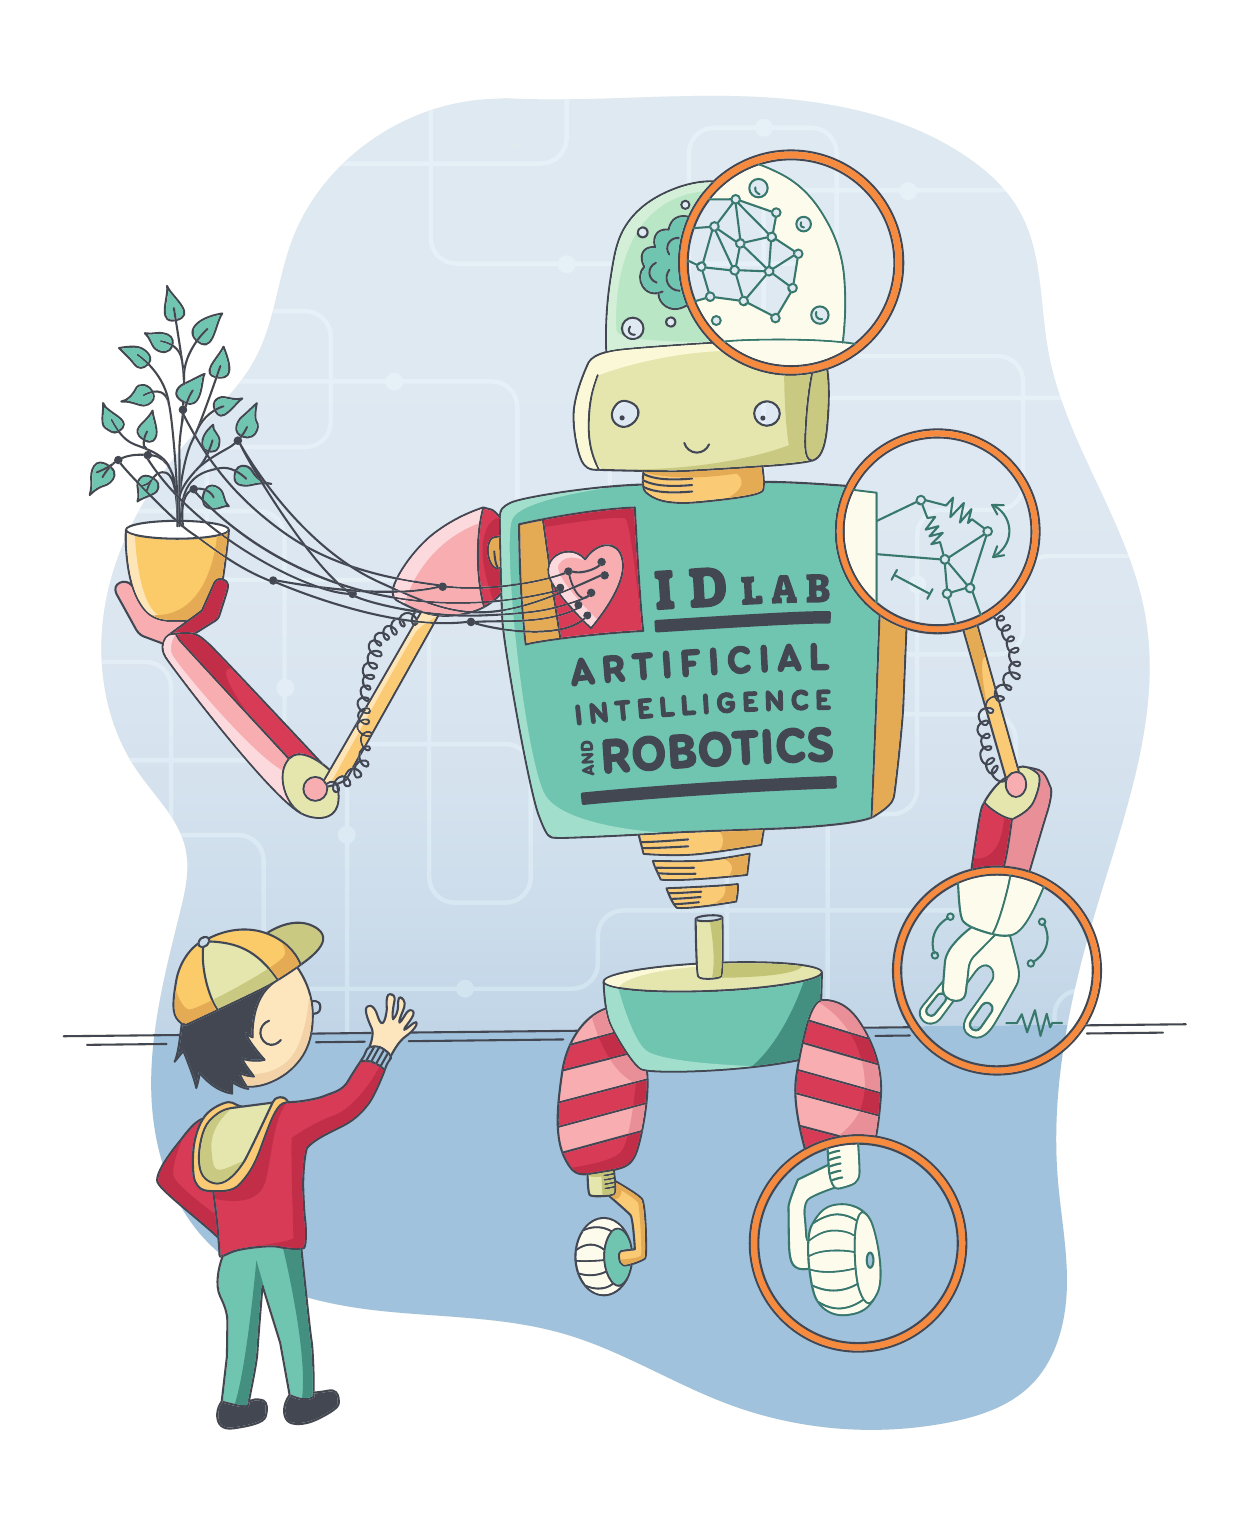
\includegraphics[width=\imwidth]{figures/AIRO} \\
%        };
%	\begin{pgfonlayer}{background}
%		\node[opacity=0.3] at ($(current page.center)+(0,0.5)$) {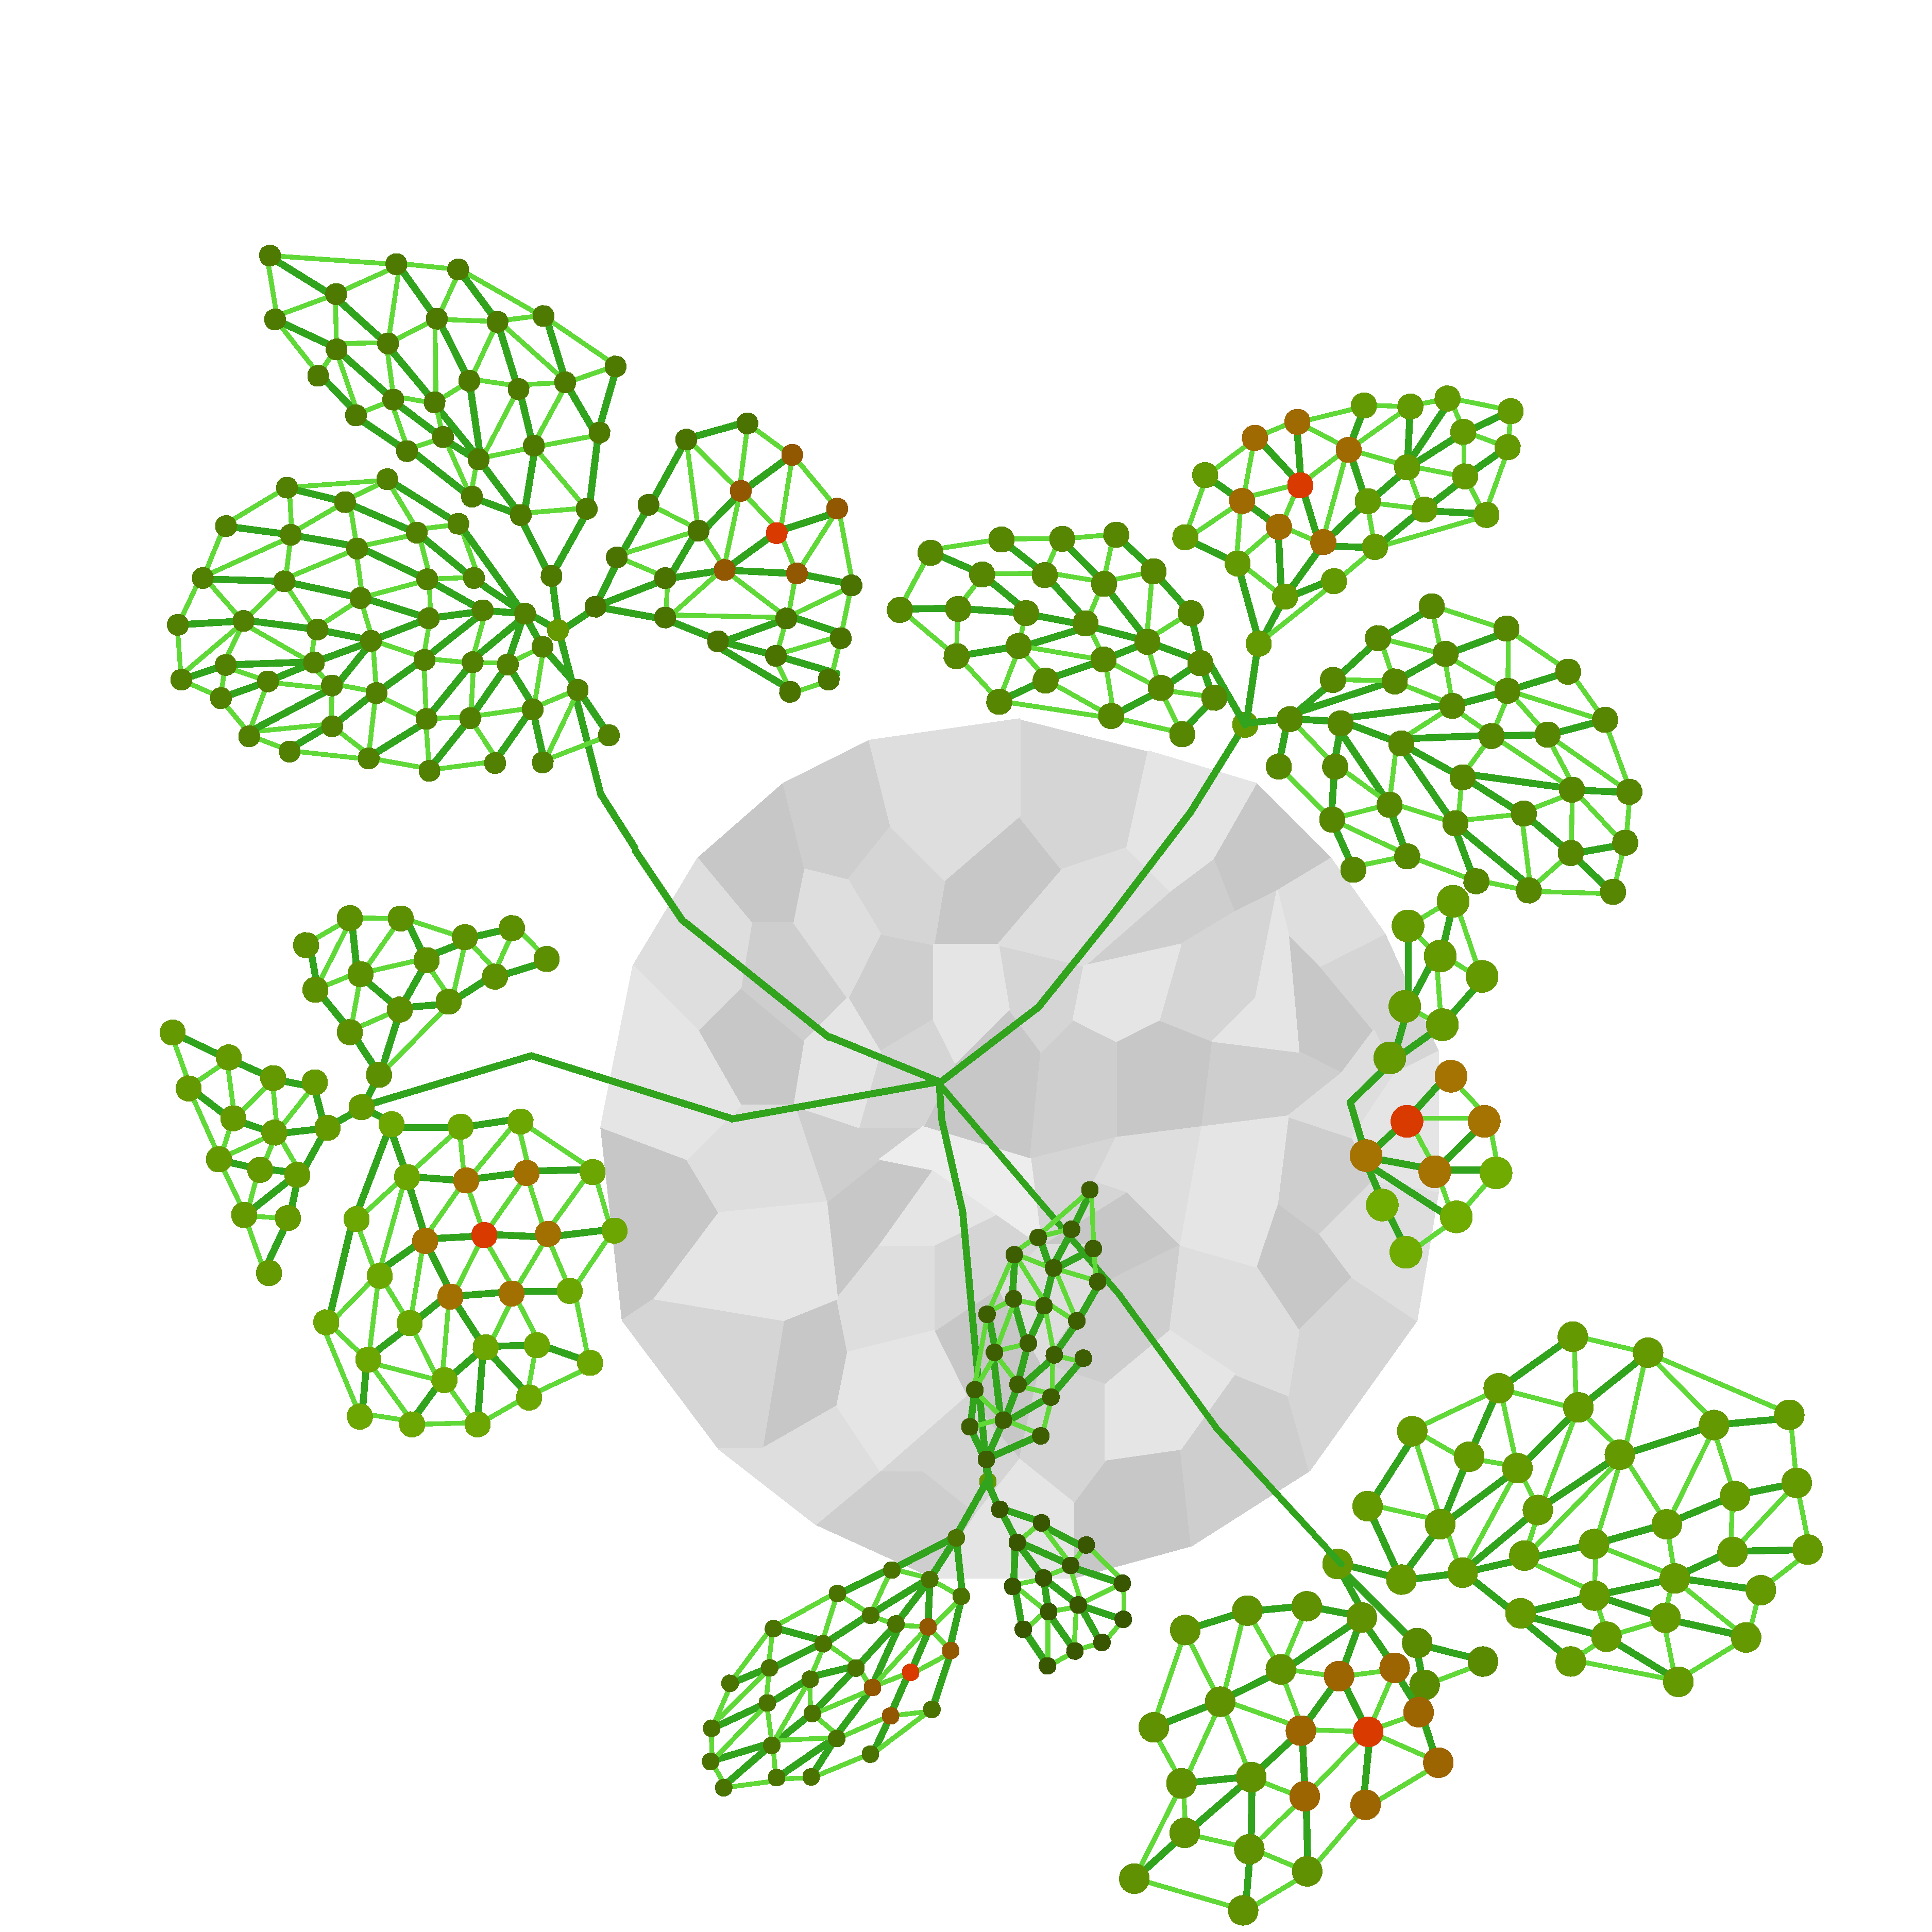
\includegraphics[height=\paperheight]{figures/bg-image}};
%	\end{pgfonlayer}
%	\end{tikzpicture}
%    \maketitle
%\end{frame}
%
%\begin{frame}{Suppose That You Want to Compare Two FSPMs}
%
%\begin{columns}
%\begin{column}{0.45\linewidth}
%\centering
%\begin{tikzpicture}
%	\node {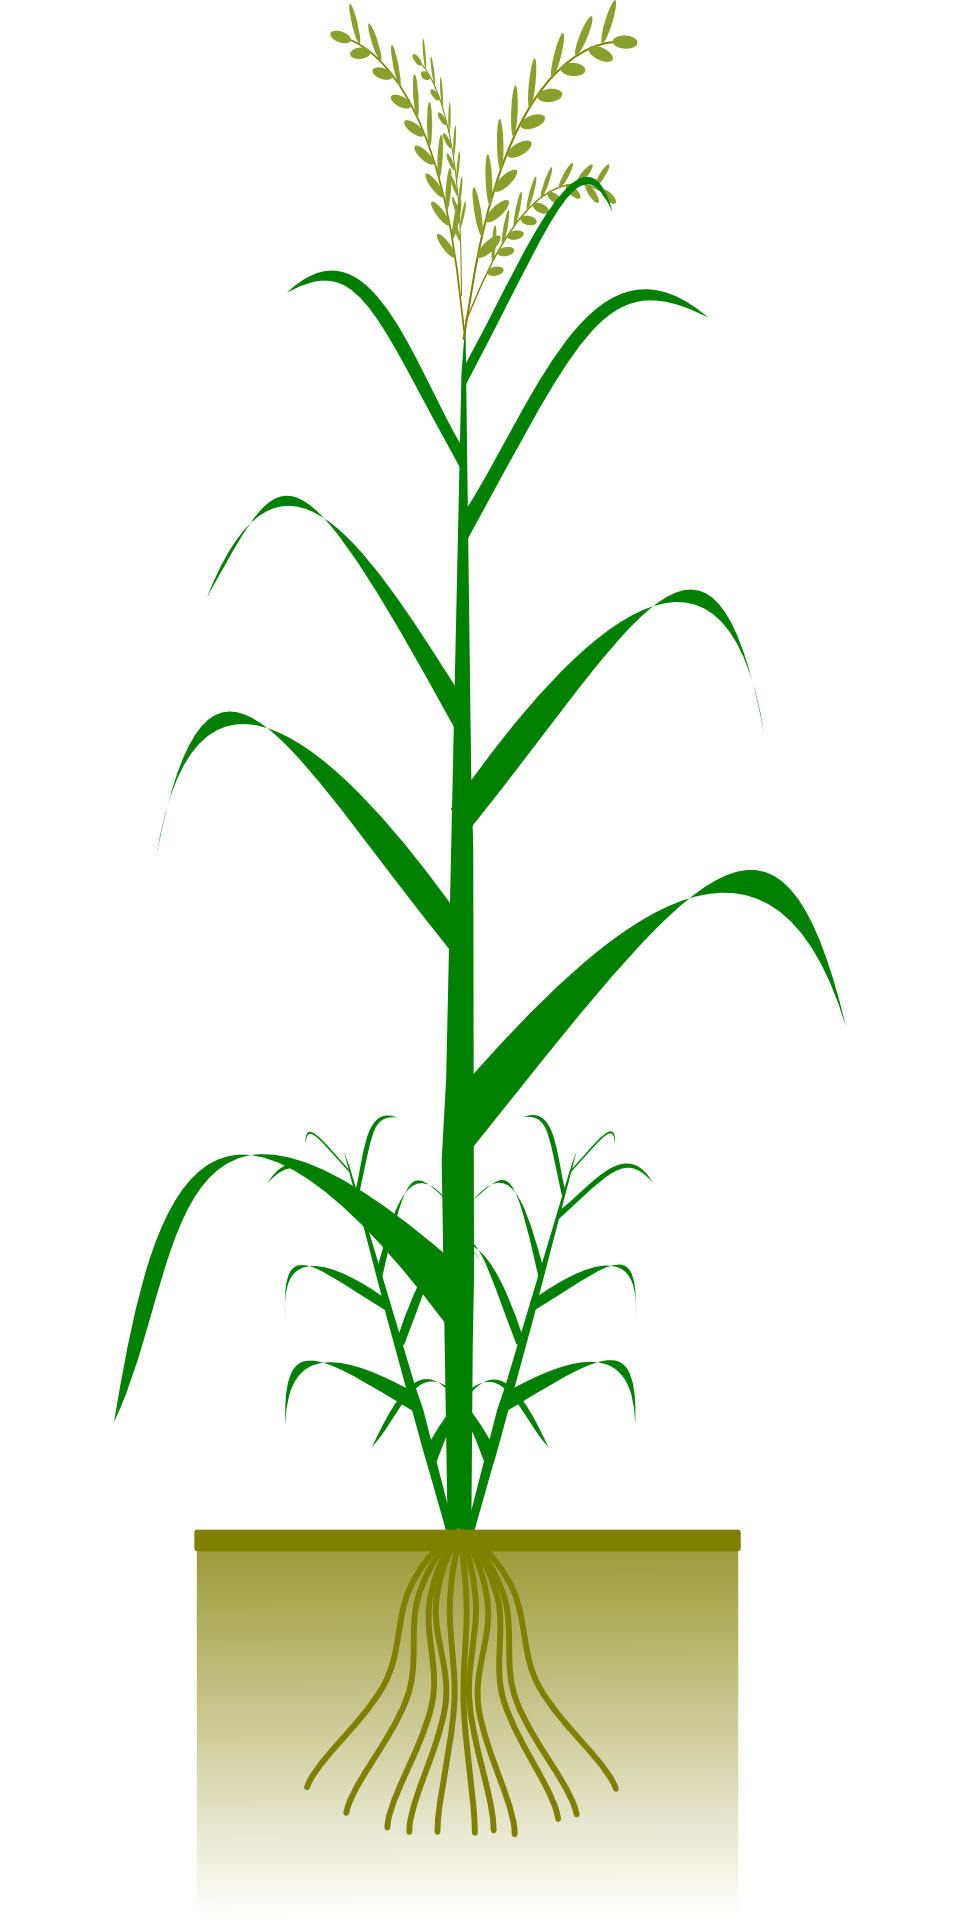
\includegraphics[width=\linewidth,height=0.7\textheight,keepaspectratio]{figures/wheat-model1}};
%	\node {\fontsize{100}{120}\selectfont A};
%\end{tikzpicture}
%\end{column}%
%\hfill%
%\begin{column}{0.45\linewidth}
%\centering
%\begin{tikzpicture}
%	\node {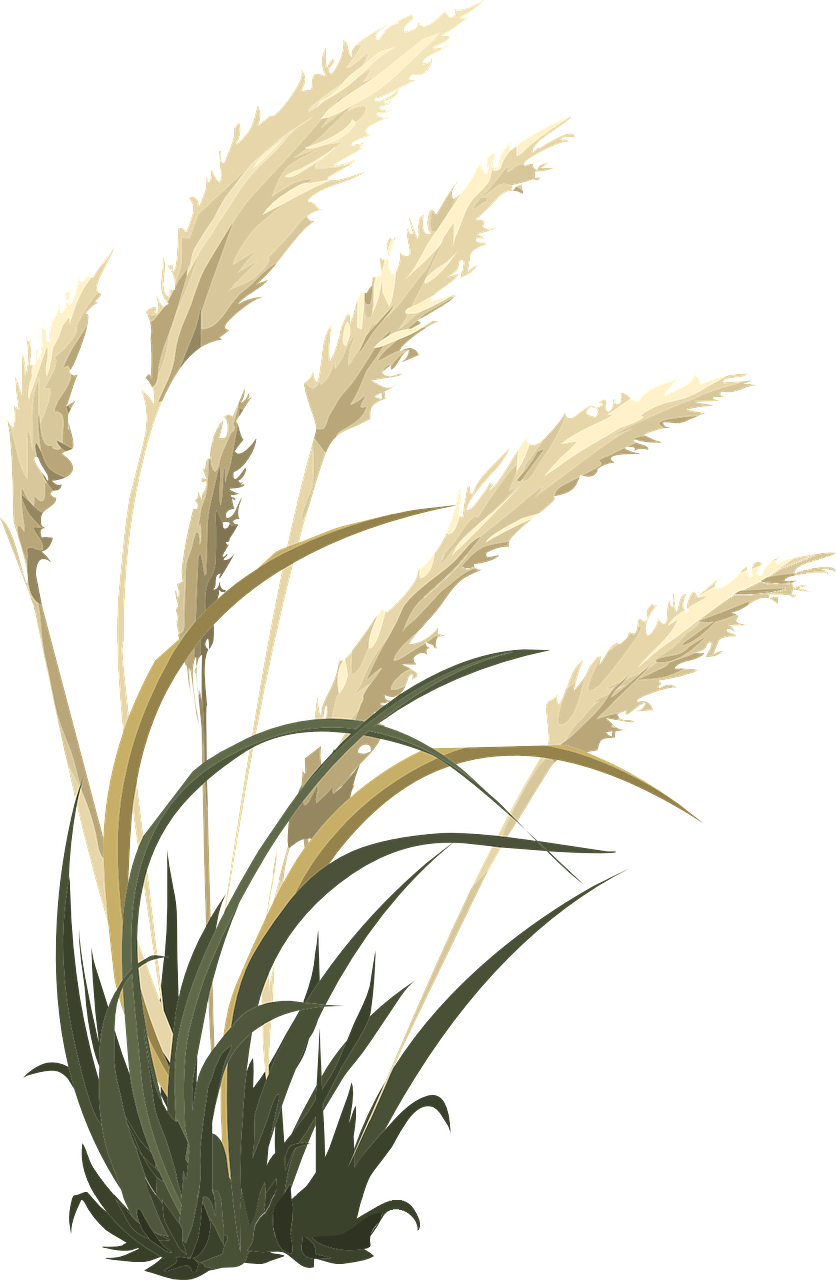
\includegraphics[width=\linewidth,height=0.7\textheight,keepaspectratio]{figures/wheat-model2}};
%	\node {\fontsize{100}{120}\selectfont B};
%\end{tikzpicture}
%\end{column}
%\end{columns}
%
%\end{frame}
%
%\begin{frame}{We Propose a New Trial-free Comparison Based on Unconventional Computing}
%
%\centering
%\begin{tikzpicture}
%
%\matrix[
%  matrix of nodes,
%  ampersand replacement=\&,
%  %column 1/.style={text width=4cm},
%  column 4/.style={text width=4cm},
%  nodes={anchor=center}
%] (m) {
%{\includegraphics[height=3cm]{figures/wheat-field}} \&[0.5cm]
%  {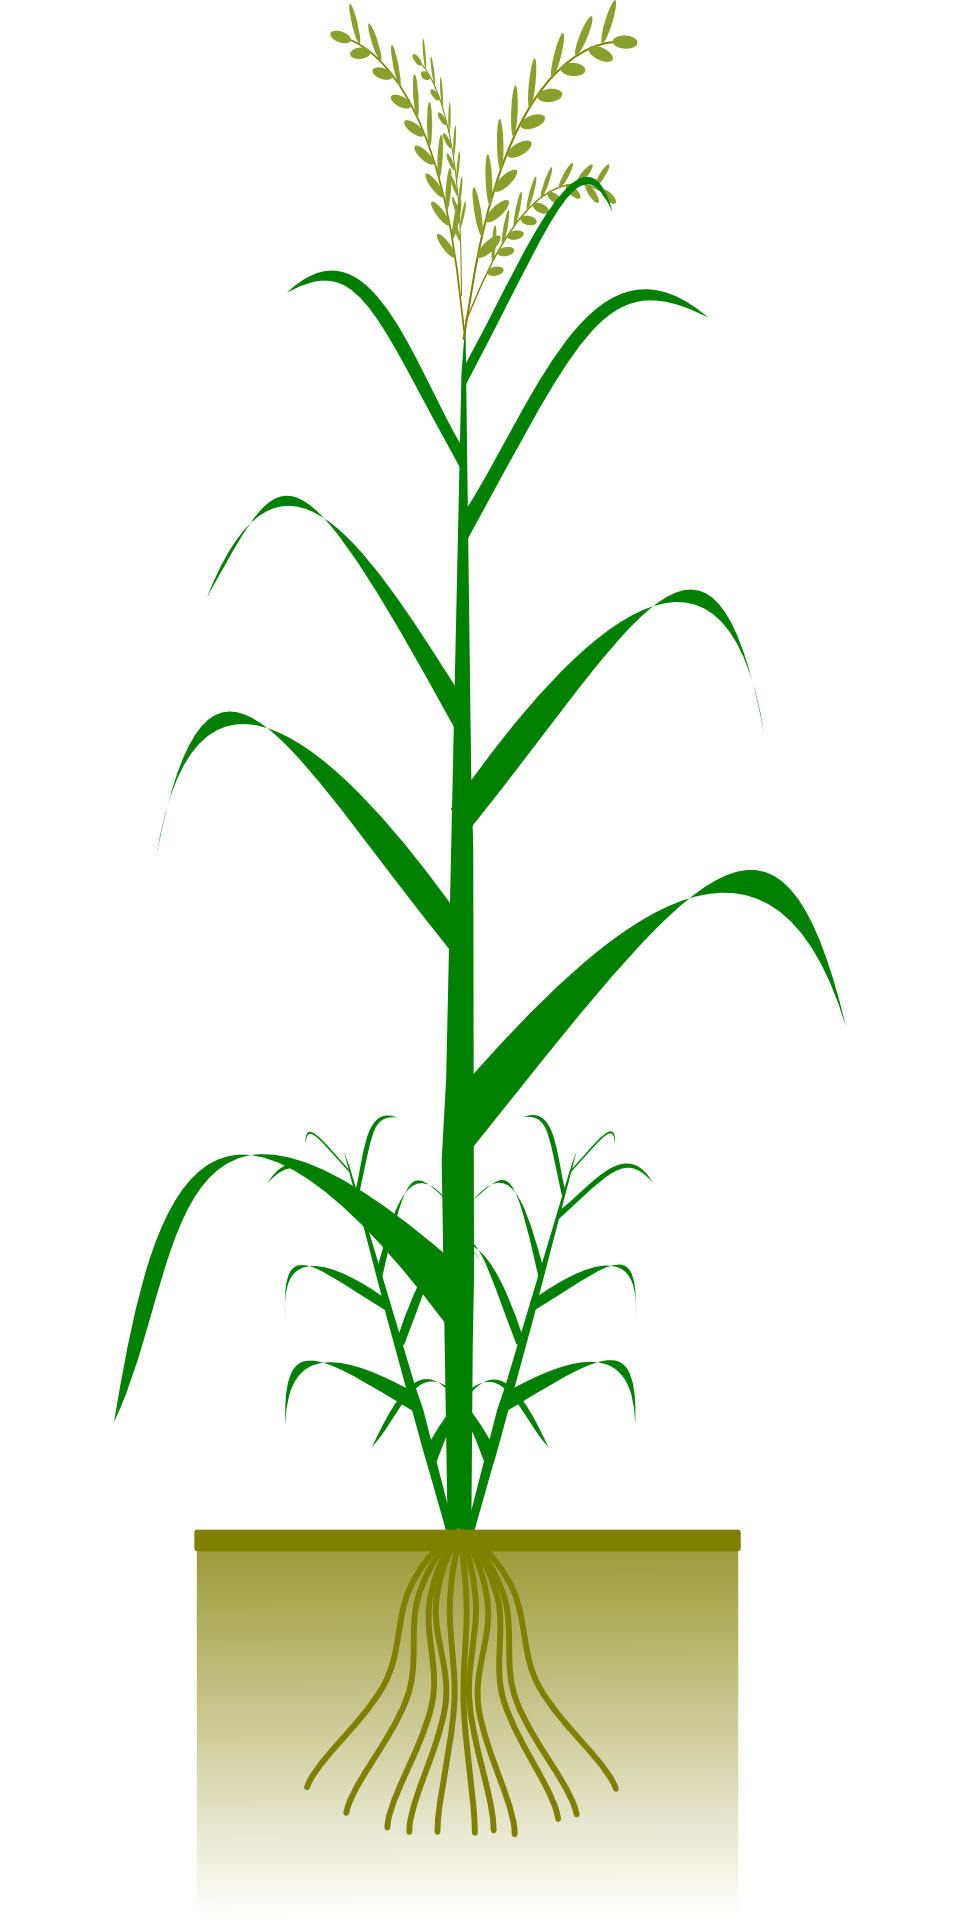
\includegraphics[height=3cm]{figures/wheat-model1}} \&
%  {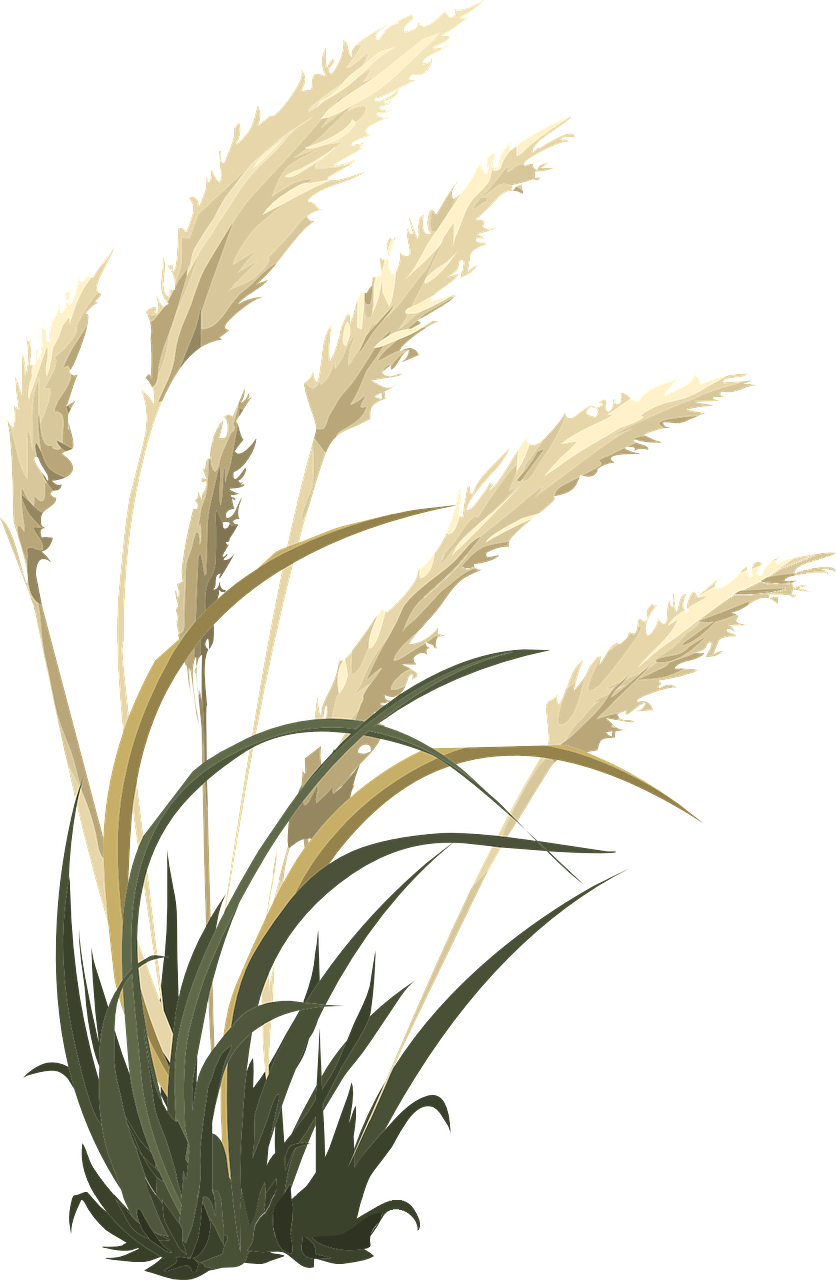
\includegraphics[height=3cm]{figures/wheat-model2}} \&[0.5cm] 
%  compare model outputs with field observations\\
%{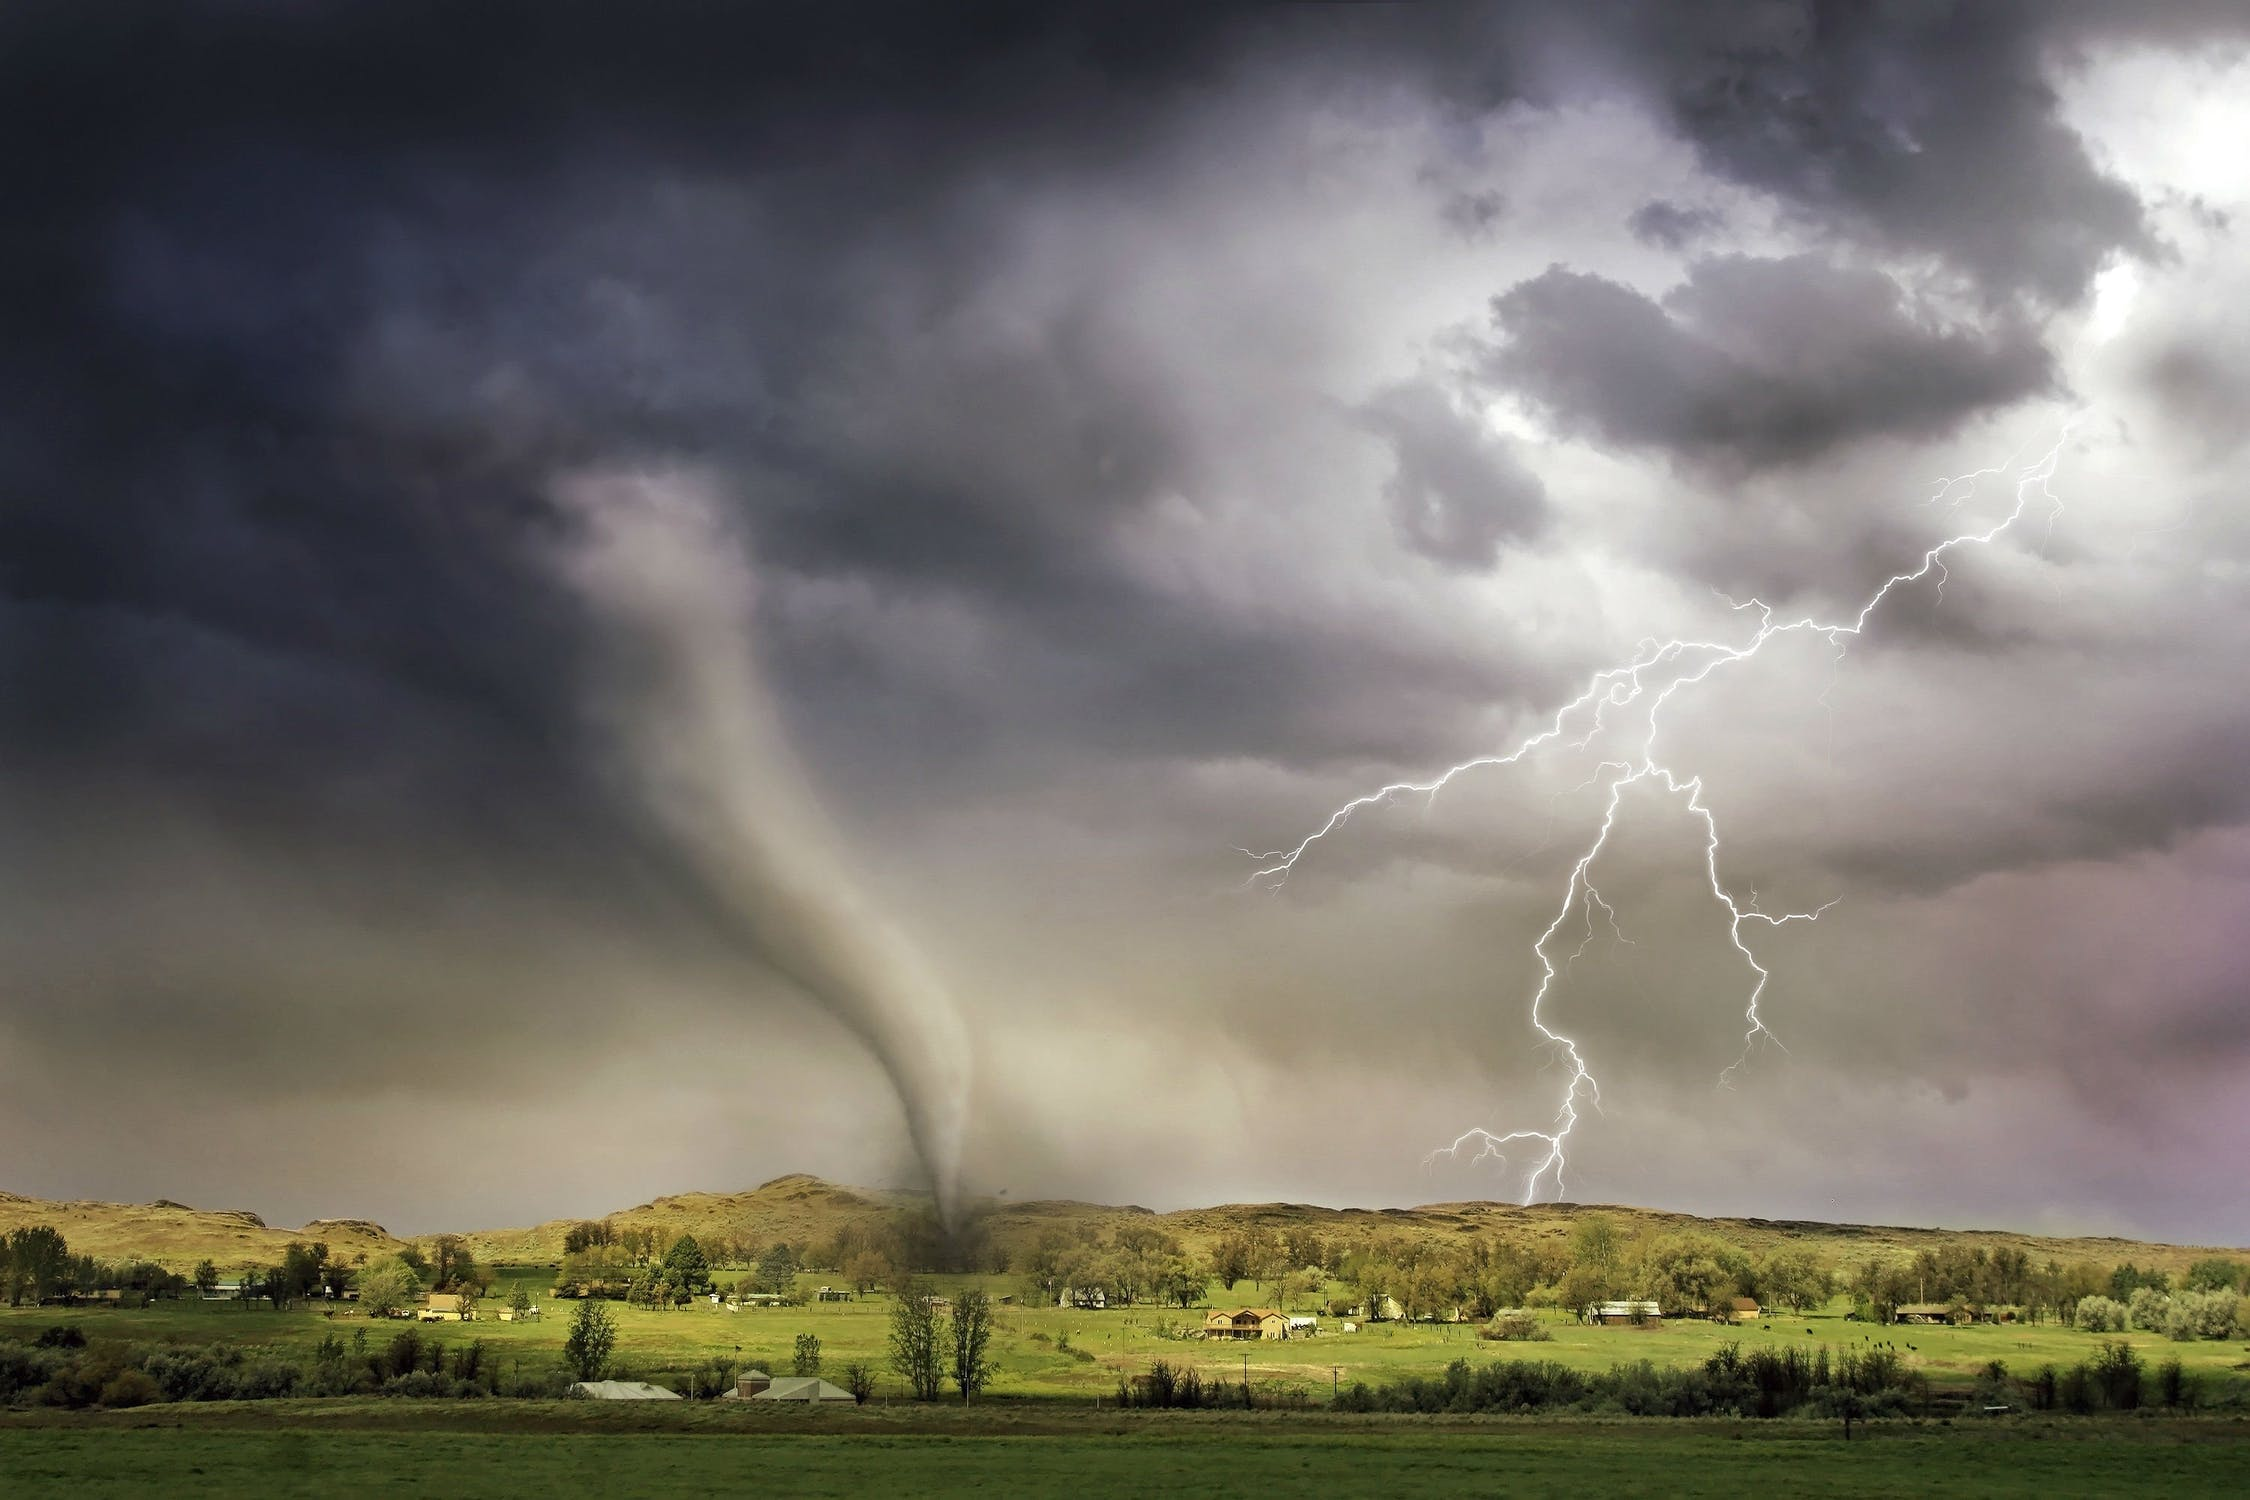
\includegraphics[height=3cm]{figures/weather}} \&
%  {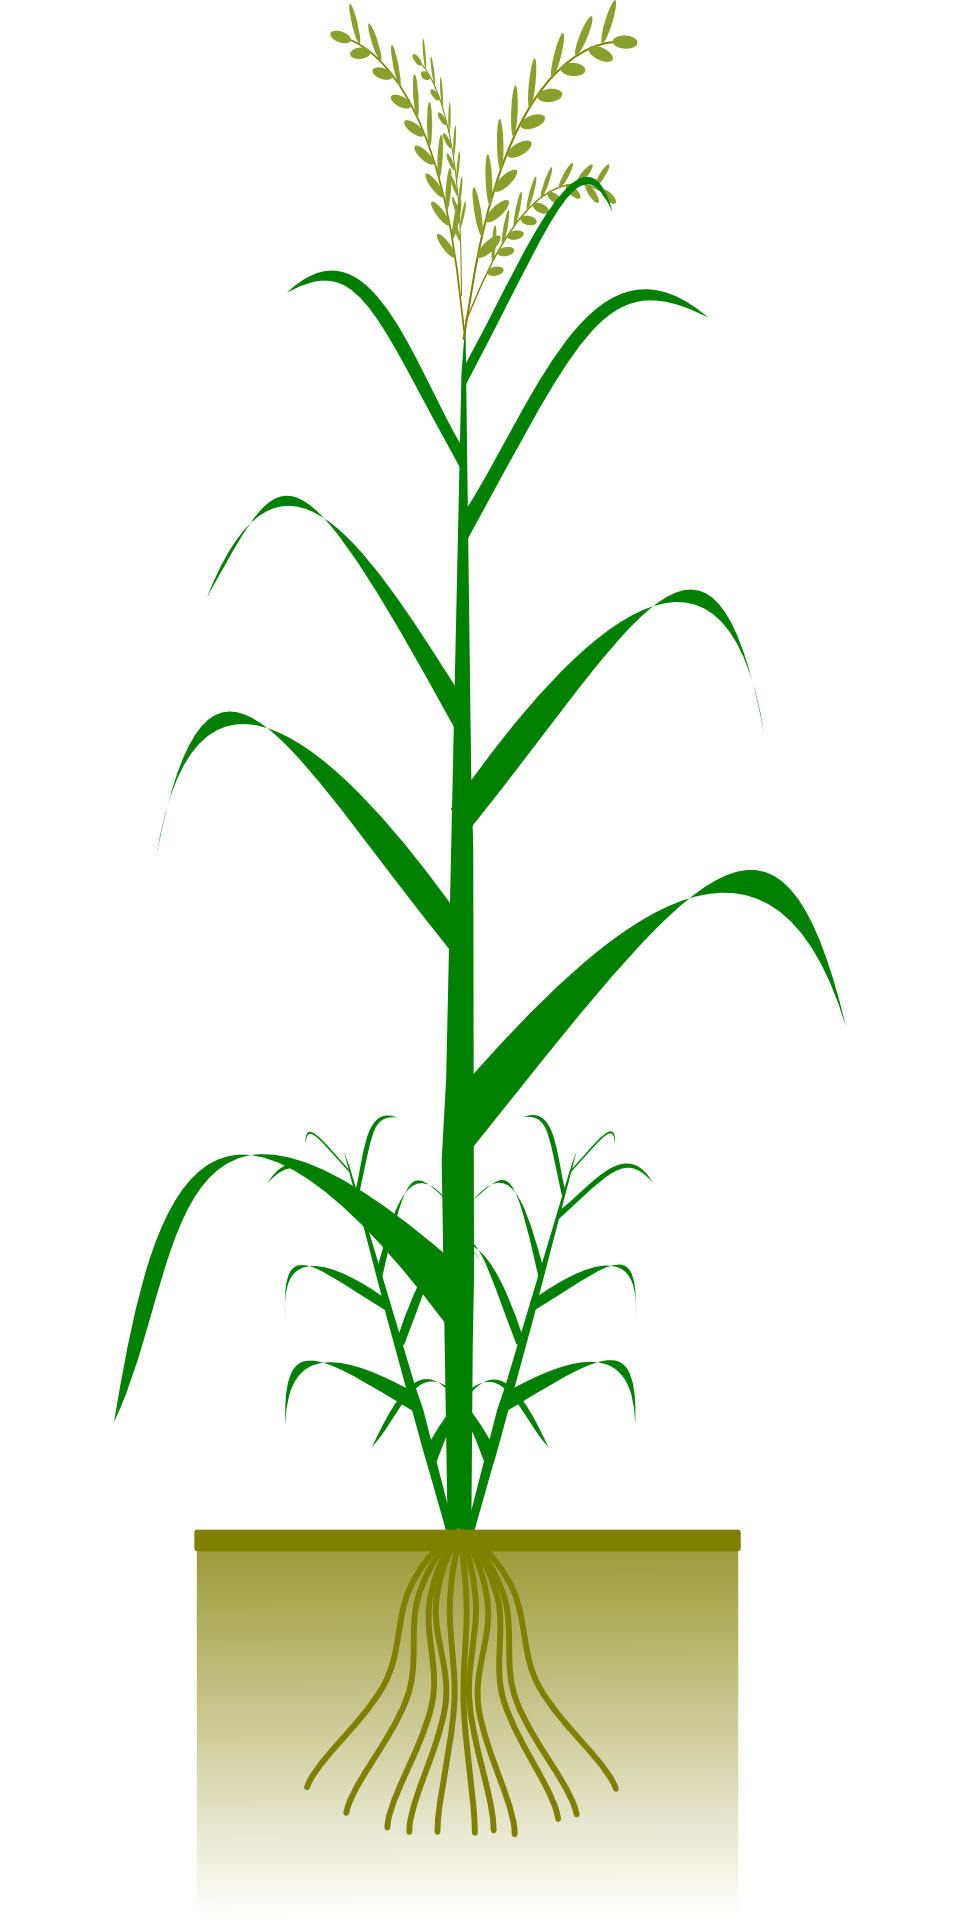
\includegraphics[height=3cm]{figures/wheat-model1}} \&
%  {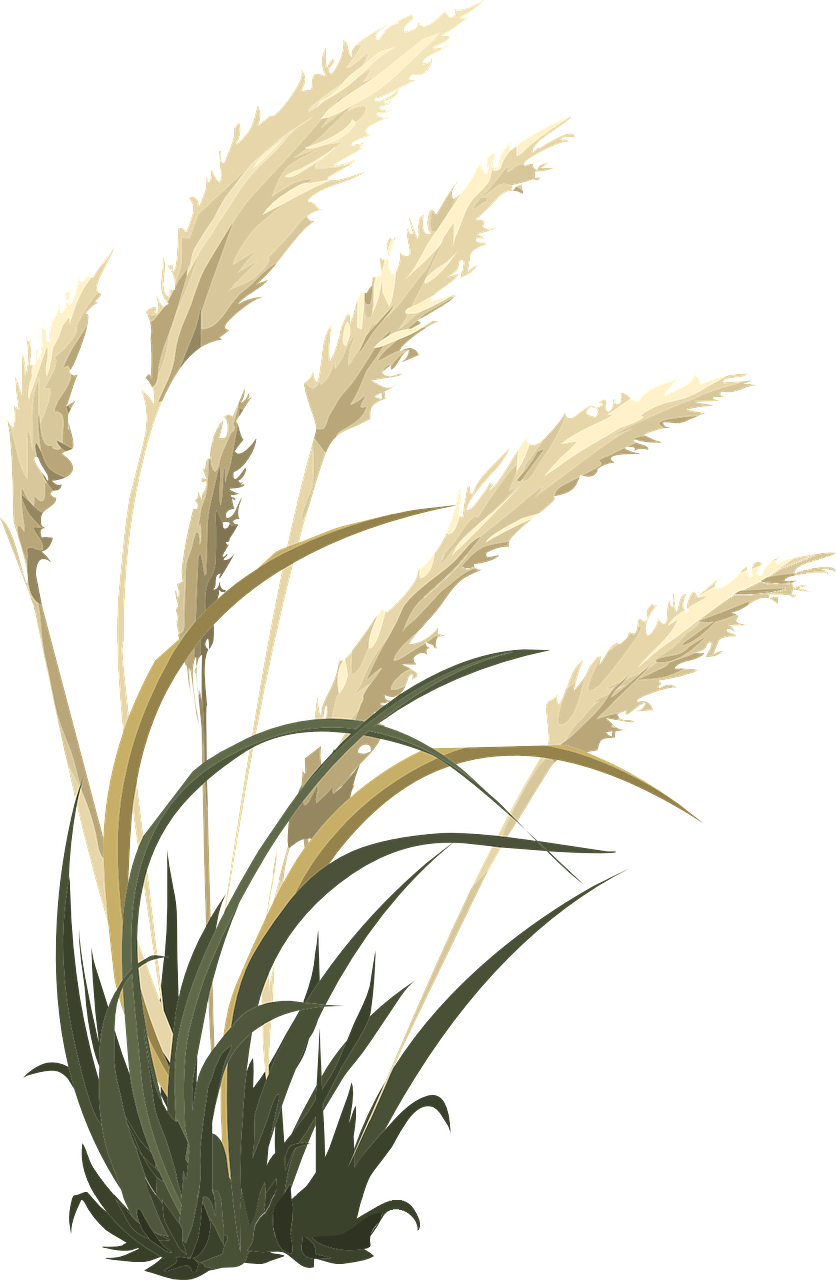
\includegraphics[height=3cm]{figures/wheat-model2}} \& 
%  input-based comparison based on model outputs\\
%};
%
%\node at (m-1-2) (mA1) {\fontsize{50}{60}\selectfont A};
%\node at (m-1-3) (mB1) {\fontsize{50}{60}\selectfont B};
%\node at (m-2-2) (mA2) {\fontsize{50}{60}\selectfont A};
%\node at (m-2-3) (mB2) {\fontsize{50}{60}\selectfont B};
%\node[anchor=north east] at (m-1-1.north east) (wobs) {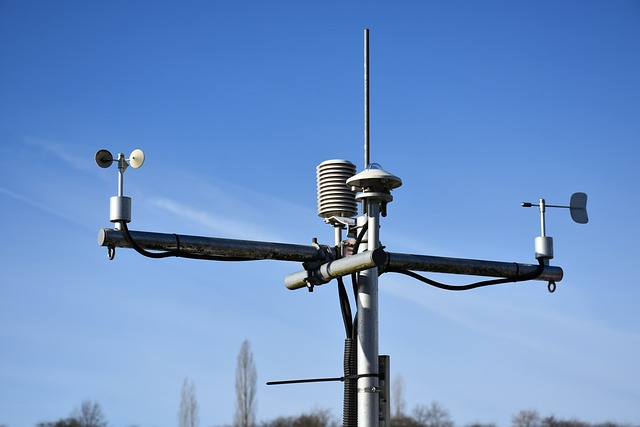
\includegraphics[height=1cm]{figures/weather-observation}};
%
%\draw[line>] (wobs.east) ++(0,0.25cm) -| (mA1);
%\draw[line>] (wobs.east) ++(0,0.25cm) -| (mB1);
%
%\draw[line>] (mA1.south) -- ++(0,-0.5cm) -| (m-1-4);
%\draw[line>] (mB1.south) -- ++(0,-0.375cm) -| ($(m-1-4.south)+(-0.5cm,0)$);
%\draw[line>] (m-1-1.south east) ++ (0,0.25cm) -| ($(m-1-4.south)+(0.5cm,0)$);
%
%\draw[line>] (m-2-1.north east) ++(0,-0.25cm) -| (mA2);
%\draw[line>] (m-2-1.north east) ++(0,-0.25cm) -| (mB2);
%\draw[line>] (m-2-1.north east) ++(0,-0.25cm) -| (m-2-4);
%
%\draw[line>] (mA2.south) -- ++(0,-0.5cm) -| ($(m-2-4.south)+(0.25cm,0)$);
%\draw[line>] (mB2.south) -- ++(0,-0.375cm) -| ($(m-2-4.south)+(-0.25cm,0)$);
%
%
%\end{tikzpicture}
%
%\end{frame}
%
%
%\begin{frame}{FSPMs Are Information Processing Systems}
%    \centering
%    \begin{tikzpicture}
%
%	\matrix[
%        matrix of nodes,
%        anchor=center,
%        inner sep=0.2em,
%		ampersand replacement=\&,
%		nodes={anchor=center},
%    ] at (-4.5,0) (input) {
%        {\color{SeqRed2}\Huge\faTemperatureLow} \& temperature \\
%        {\color{SeqBlue2}\Huge\faTint}          \& \node[align=center]{humidity\\ water availability}; \\
%        {\color{orange}\Huge\faSun}         \& light \\
%    };
%
%    \node[anchor=center,inner sep=0pt] at (0,0) (image) {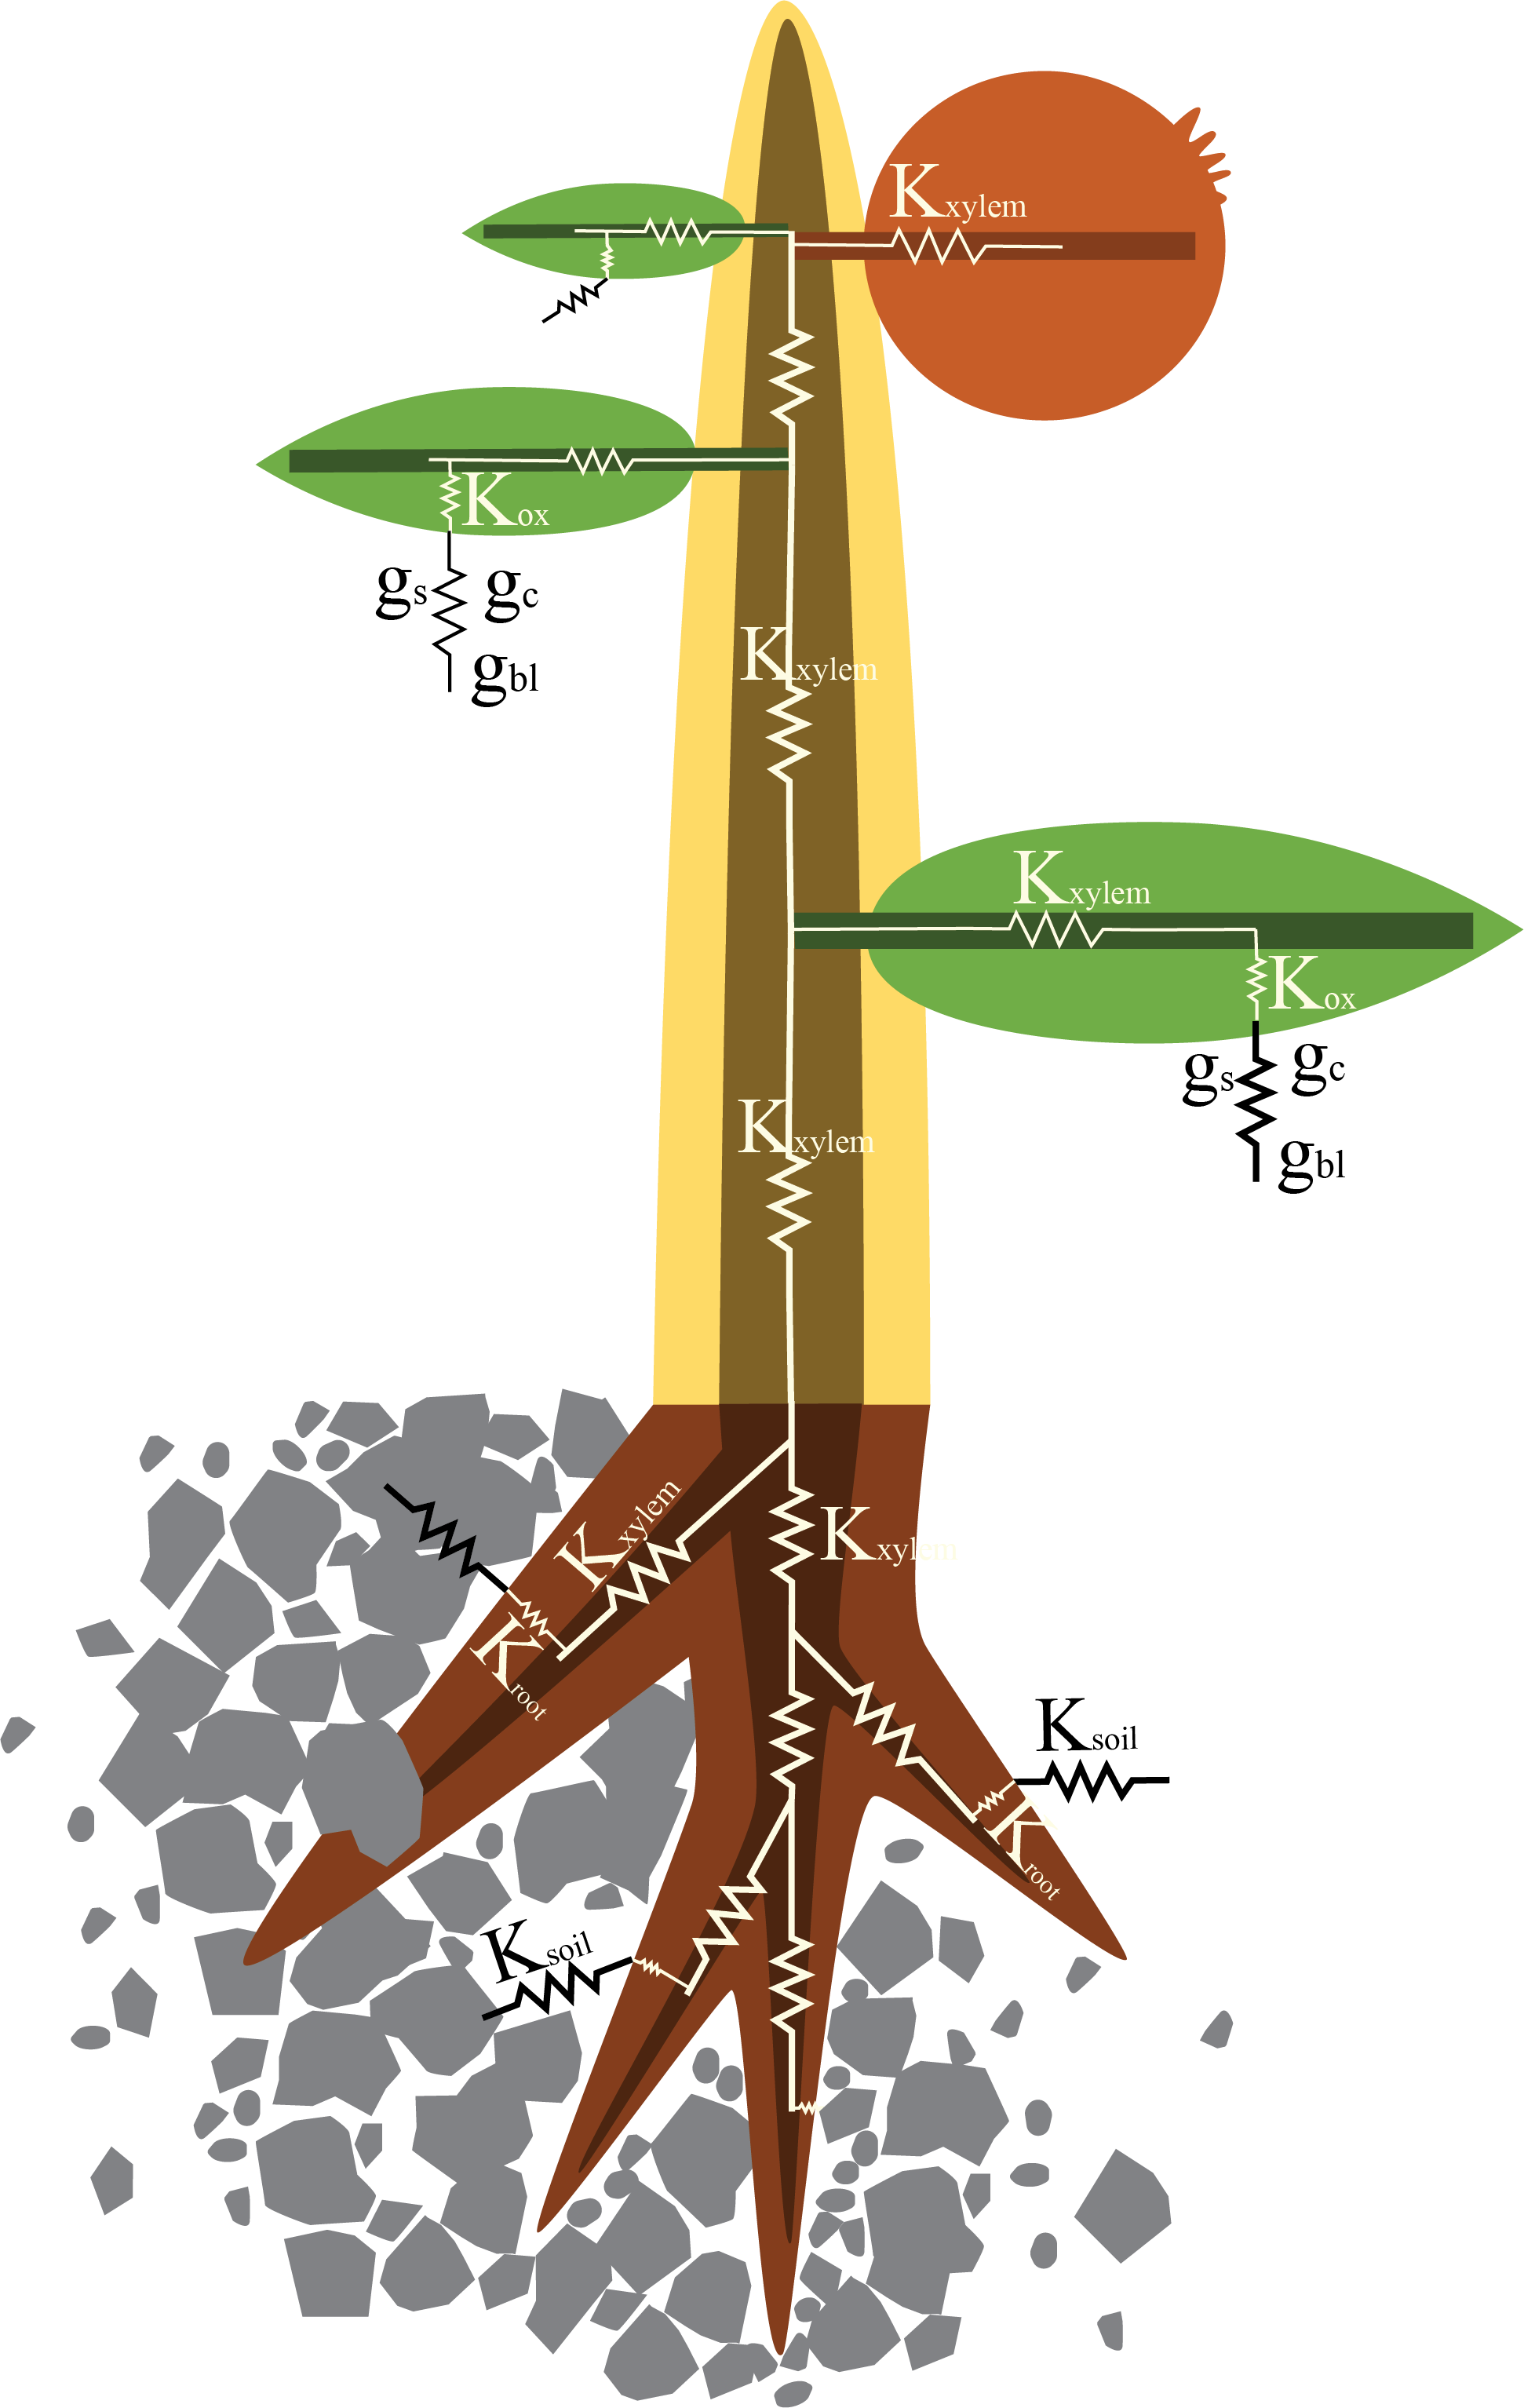
\includegraphics[height=6cm]{figures/plant-model}};
%
%	\matrix[
%        matrix of nodes,
%        anchor=center,
%        inner sep=0.2em,
%		ampersand replacement=\&,
%		nodes={anchor=center},
%    ] at (4.5,0) (output) {
%        {\color{SeqRed2}\Huge\faTemperatureLow} \& surface temperature \\
%        {\color{SeqBlue2}\Huge\faTint}          \& \node[align=left]{transpiration rate\\water flow\\water potential}; \\
%        {\color{orange}\Huge\faSun}         \& net photosynthesis \\
%    };
%
%
%	\begin{scope}[transparency group,-{Latex[length=10mm, width=12.5mm]},,opacity=0.3]
%		\draw[line width=5mm] ($0.5*(input.east)+0.5*(input.center)$) -- ($0.5*(image.west)+0.5*(image.center)$);
%		\draw[line width=5mm] ($0.5*(image.east)+0.5*(image.center)$) -- ($0.5*(output.west)+0.5*(output.center)$);
%	\end{scope}
%	
%	\only<2->{%
%	\begin{scope}[every node/.style={fill=white,fill opacity=0.85,text opacity=1,text=fg,minimum height=3cm,minimum width=3.5cm}]
%	  \node at (input.center) {\Huge \textbf{inputs}};
%	  \node at (image.center) (processing) {\Huge \textbf{processing}};
%	  \node at (output.center) {\Huge \textbf{outputs}};
%    \end{scope}
%	}
%    \only<3->{%
%	\begin{scope}[every node/.style={fill=white,fill opacity=0.85,text opacity=1,text=fg}]
%	  \node [above left=0.6cm and 3cm of processing.north,anchor=base] {\huge non-linear};
%	  \node [above right=0.6cm and 3cm of processing.north,anchor=base] {\huge memory};
%    \end{scope}
%    	}
%
%    \only<4->{%
%	\begin{scope}[every node/.style={fill=white,fill opacity=0.85,text opacity=1,text=fg}]
%	  \node [below=0.5cm of processing.south] {\Huge \textbf{reservoir computing}};
%    \end{scope}
%    	}
%
%    \end{tikzpicture}
%\end{frame}
%
%\begin{frame}{Reservoir Computing Enables Computing with Dynamic Systems}
%    \centering
%    \begin{tikzpicture}
%    
%    	% draw rectangle labels
%    	\node[box label,anchor=base] at (1,3.5) (i-label) {input};
%    	\node[box label,anchor=base] at (5,3.5) (res-label) {reservoir/RNN};
%    	\node[box label,anchor=base] at (9,3.5) (o-label) {target};
%    	
%    	\draw[line] (i-label.base) ++(-1,-0.2) -- ++(2,0);
%    	\draw[line] (res-label.base) ++(-2.5,-0.2) -- ++(5,0);
%    	\draw[line] (o-label.base) ++(-1,-0.2) -- ++(2,0);
%    	
%    	
%    	%%% other reservoir
%  	\begin{scope}
%      \node[input node] at (1,2) (in0) {};
%      \node[input node] at (1,1) (in1) {};
%
%    	\setcounter{resnode}{0}
%    	% reservoir nodes
%    	\foreach \x/\y in {3/2.25,3.5/1,4/3.5,5/1.5,5.25/3.75,6/0.5,6.15/2.25,7/3.5} {
%    		\draw (\x,2.5*\y/3.5) node[reservoir node] (rn\the\value{resnode}) {};
%    		\stepcounter{resnode}
%    	}
%
%    	% input arrows
%    	\foreach \i/\j in {0/0,0/1,1/0,1/2} {
%    		\draw[line>] (in\i) -- (rn\j);
%    	}
%
%    	% reservoir arrows
%    	\foreach \i/\j in {0/3,0/2,1/0,1/5,2/1,3/1,2/3,4/2,5/6,6/2,6/4,6/7,7/0,7/4} {
%    		\draw[line>] (rn\i) -- (rn\j);
%    	}
%    	% bent arrows
%        \foreach \i/\j in {2/0,5/7} {
%       		\draw[line>] (rn\i) to[bend right] (rn\j);
%       	}
%       	
%    
%        	% output nodes
%    	\node[output node] at (9,1.5) (out0) {};
%
%    	% output arrows
%    	\draw[line>,red2] (rn6) -- (out0);
%       	\draw[line>,red2] (rn3) -- (out0);
%       \draw[line>,red2] (rn5) -- (out0);
%       \draw[line>,red2] (rn7) -- (out0);
%       \end{scope}
%	\end{tikzpicture}
%	
%	\tikz{
%	\matrix[
%		matrix of nodes,
%		column sep=0.2cm,
%		ampersand replacement=\&,
%		] {
%	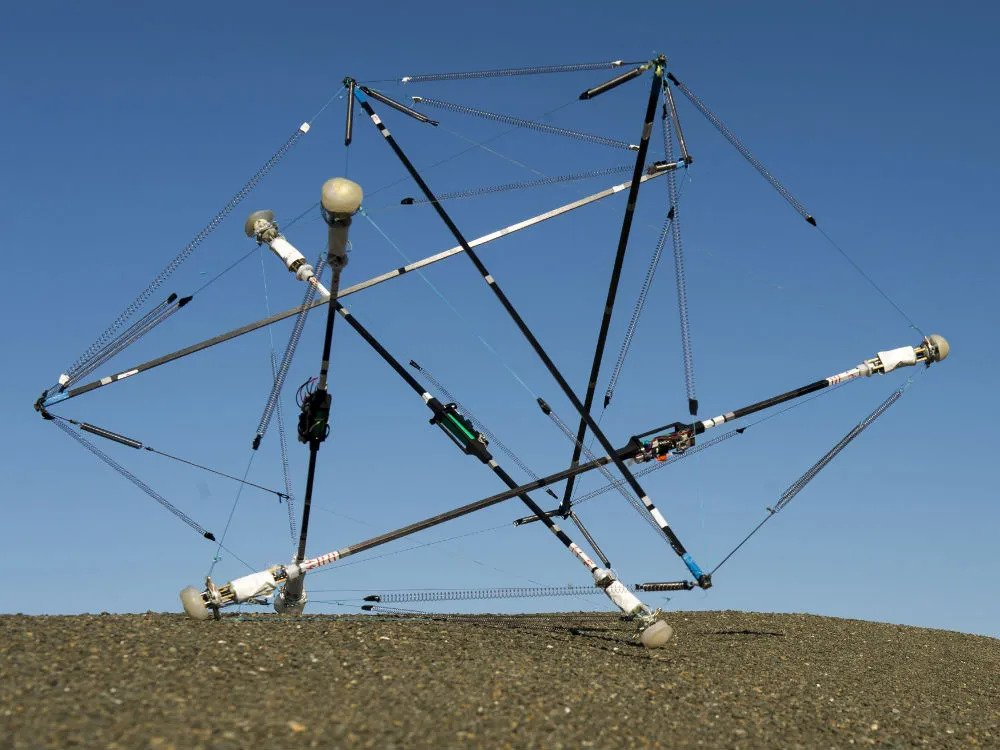
\includegraphics[height=2cm]{figures/nasa-ball-robot} \&
%	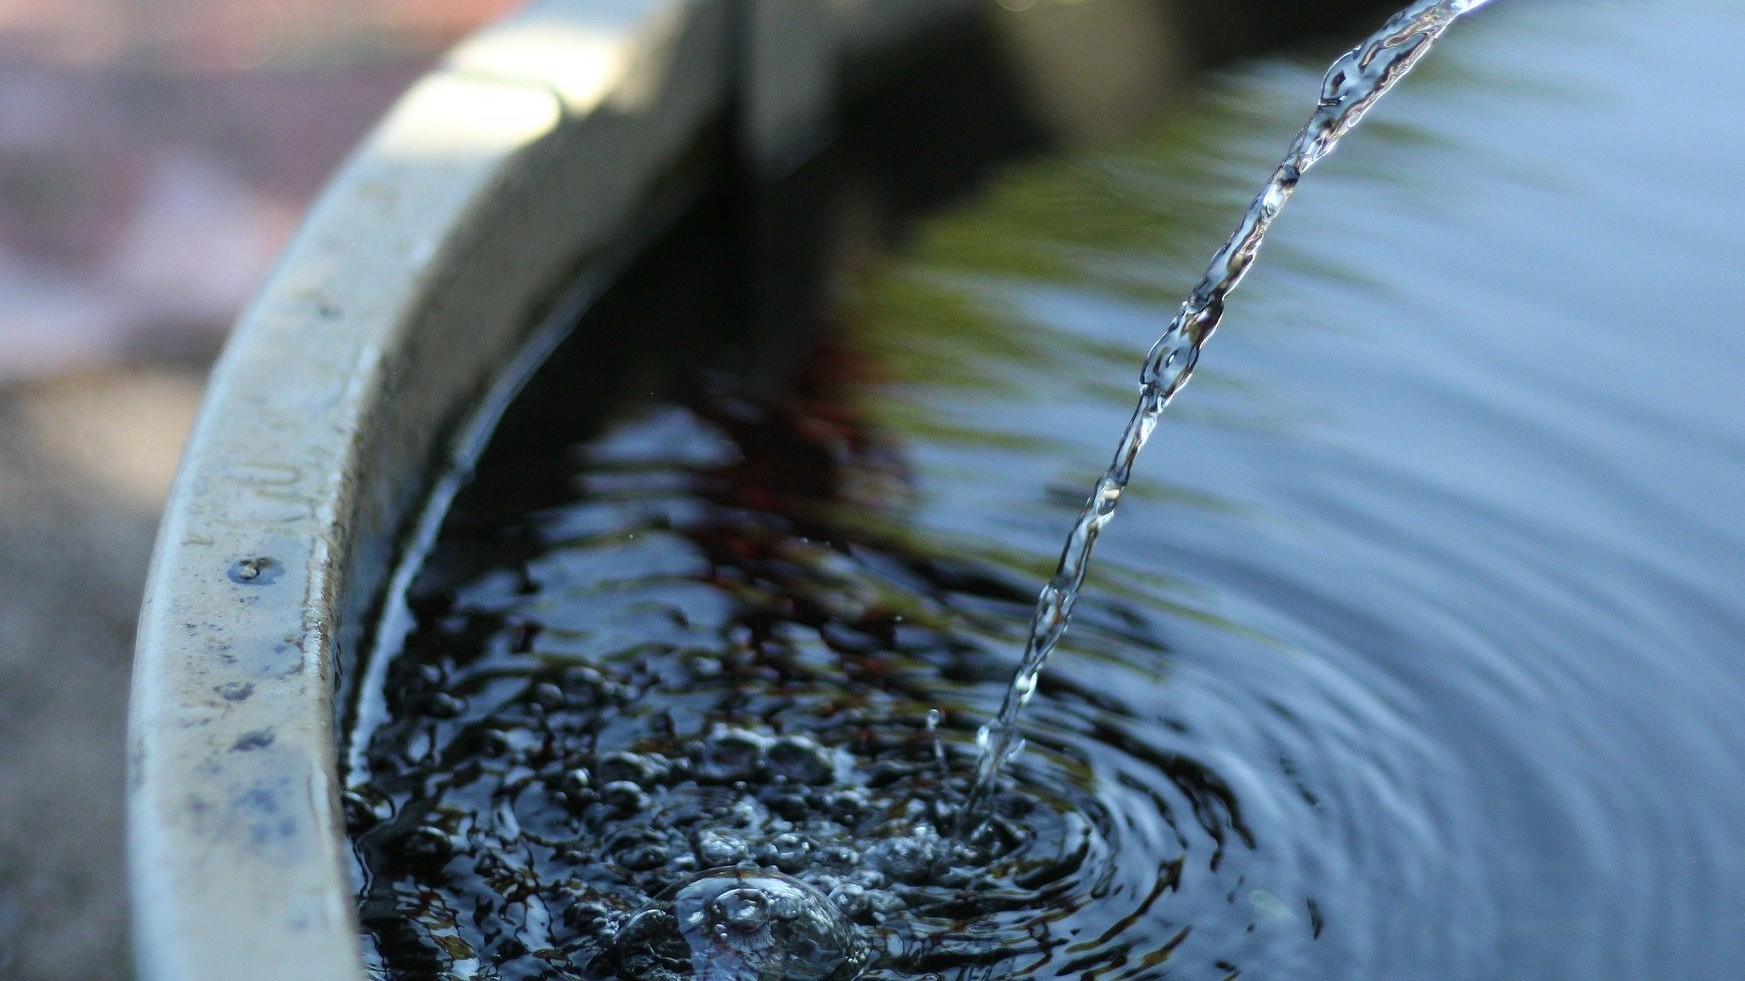
\includegraphics[height=2cm]{figures/water_bucket_ripples} \&
%	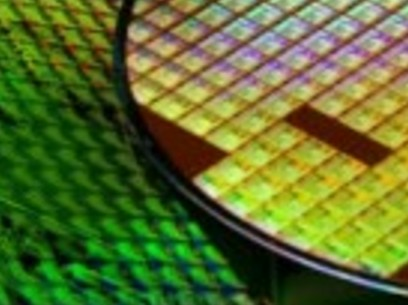
\includegraphics[height=2cm]{figures/photinic_ic} \&
%	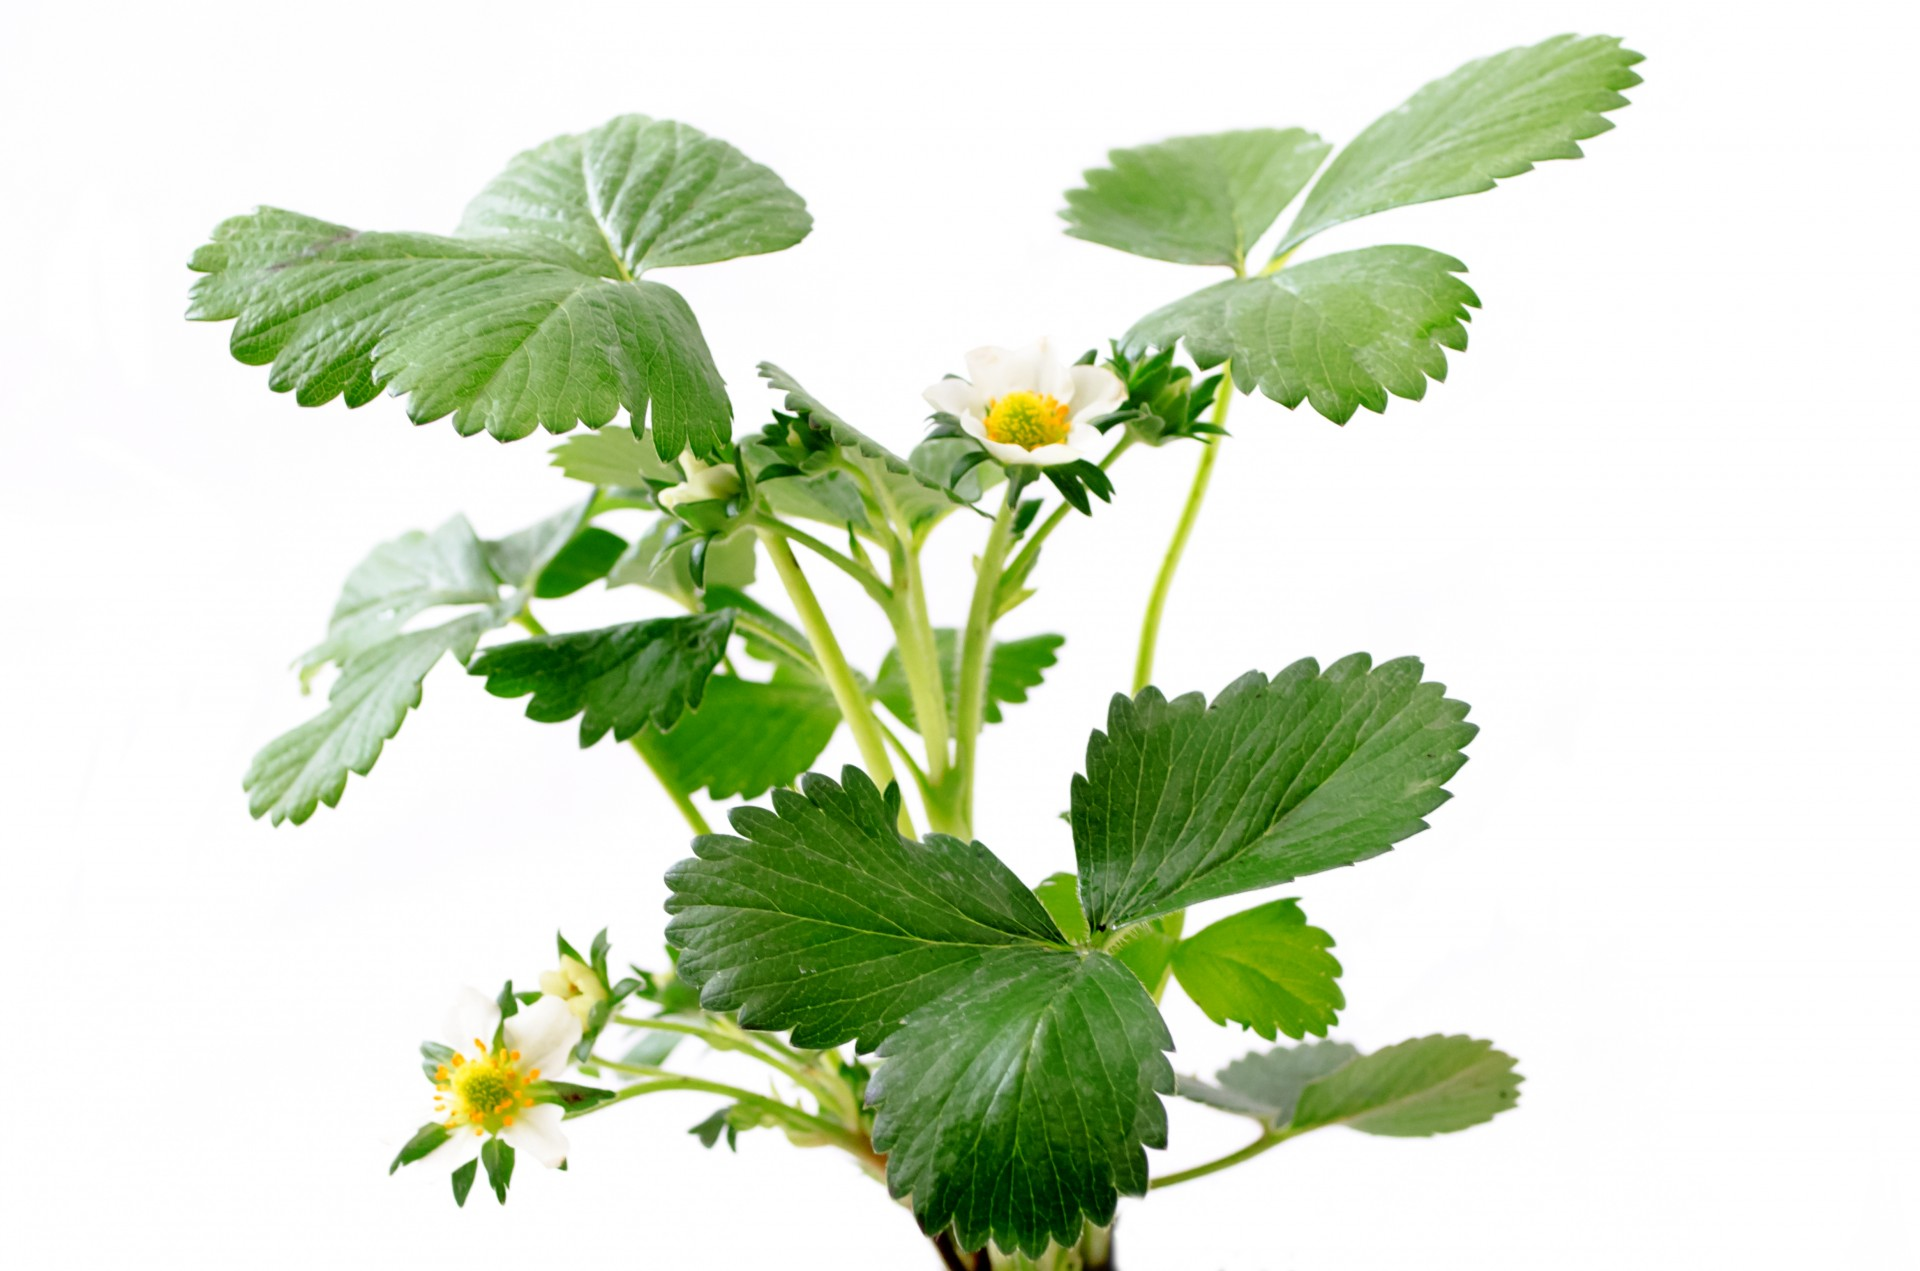
\includegraphics[height=2cm]{figures/strawberry}\\
%	};
%	}
%	
%\end{frame}


\begin{frame}{Reservoir Computing Applied to FSPMs}
    \centering
    \begin{tikzpicture}
    	% rectangles
    	\draw[box] (0,0) rectangle (2,6);
    	\draw[box] (2.5,0) rectangle (7.5,6);
    	\draw[box] (8,0) rectangle (10,6);

    	% draw rectangle labels
    	\node[box label,anchor=base] at (1,6.2) {input};
    	\node[box label,anchor=base] at (5,6.2) {reservoir};
    	\node[box label,anchor=base] at (9,6.2) {target};
    	
    	%% draw plant reservoir
    	
    	% draw sun, rain and bug
    	\node at (0.5,4) {\color{orange}\huge\faSun};
    	\node at (1.5,4) {\color{blue}\huge\faCloudShowersHeavy};
    	\node at (1,5) {\huge\faBug};
    	

    	% draw plant
    	\draw[postaction={decorate,
    		decoration={
    			markings,
    			mark=between positions 0.2 and 0.9 step 0.45 with {
    				\draw[line width=1pt,SeqGreen2,fill=SeqGreen3,line cap=round] (0,0) to[bend right,looseness=1.2] (.575,-0.46);
    				\draw[line width=1pt,SeqGreen2,fill=SeqGreen3,line cap=round] (0,0) to[bend left,looseness=1.2] (.575,-0.46);
    				\draw[line width=1pt,SeqGreen2,line cap=round] (0,0) -- (0.425,-0.34);
        	}}},
        	postaction={decorate,
        		decoration={
        			markings,
        			mark=between positions 0.4 and 0.5 step 0.2 with {
        				\draw[line width=1pt,SeqGreen2,fill=SeqGreen3,line cap=round] (0,0) to[bend right,looseness=1.2] (.575,0.46);
        				\draw[line width=1pt,SeqGreen2,fill=SeqGreen3,line cap=round] (0,0) to[bend left,looseness=1.2] (.575,0.46);
        				\draw[line width=1pt,SeqGreen2,line cap=round] (0,0) -- (0.425,0.34);
        			}
        	}},
        	SeqGreen2,line width=1.5pt,line cap=round]
    	   (5,4) to[out=90,in=-75] ++(-0.5,2);
    	% draw pot
    	\draw[brown,fill=brown] (5,3.25) -- ++(-0.5,0) -- ++(-0.1,0.75) -- ++(1.2,0) -- ++(-0.1,-0.75) -- cycle;

    	% output    	
    	\draw (7,3.2) node[anchor=center] (leaf) {\Large\color{SeqGreen2}\faLeaf};
        \draw (7,4.1) node[anchor=center] (rh) {\Large\color{SeqRed2}\faApple*};
        \draw (7,4.9) node[anchor=center] (carrot) {\Large\color{SeqYellow2}\faCarrot};
        \draw (7,5.6) node[anchor=center] (carrot) {\Large\color{SeqYellow2}\color{SeqGrey2}\faEyeDropper};
        
        \node[output node] at (9,4.5) (fspm-target) {};

    	\draw[line>] (1.9,4.5) -- (4.5,4.5);
    	\draw[line>] (5.5,4.2) -- (6.6,3.2);
    	\draw[line>] (5.5,4.4) -- (6.6,4.1);
    	\draw[line>] (5.5,4.6) -- (6.6,4.9);
    	\draw[line>] (5.5,4.8) -- (6.6,5.6);
    	\draw[line>] (7.3,4.5) -- (fspm-target) node[midway,above,text=fg,fill=BgColor,fill opacity=0.90,text opacity=1] {\Large ?};
    	%\draw[line>] (7,-2.25) -- (rh);
    	
    	%%% other reservoir
  	\begin{scope}
      \node[input node] at (1,2) (in0) {};
      \node[input node] at (1,1) (in1) {};

    	\setcounter{resnode}{0}
    	% reservoir nodes
    	\foreach \x/\y in {3/2.25,3.5/1,4/3.5,5/1.5,5.25/3.75,6/0.5,6.15/2.25,7/3.5} {
    		\draw (\x,2.5*\y/3.5) node[reservoir node] (rn\the\value{resnode}) {};
    		\stepcounter{resnode}
    	}

    	% input arrows
    	\foreach \i/\j in {0/0,0/1,1/0,1/2} {
    		\draw[line>] (in\i) -- (rn\j);
    	}

    	% reservoir arrows
    	\foreach \i/\j in {0/3,0/2,1/0,1/5,2/1,3/1,2/3,4/2,5/6,6/2,6/4,6/7,7/0,7/4} {
    		\draw[line>] (rn\i) -- (rn\j);
    	}
    	% bent arrows
        \foreach \i/\j in {2/0,5/7} {
       		\draw[line>] (rn\i) to[bend right] (rn\j);
       	}
       	
    
        	% output nodes
    	\node[output node] at (9,1.5) (out0) {};

    	% output arrows
    	\draw[line>,red2] (rn6) -- (out0);
       	\draw[line>,red2] (rn3) -- (out0);
       \draw[line>,red2] (rn5) -- (out0);
       \draw[line>,red2] (rn7) -- (out0);
       \end{scope}
	\end{tikzpicture}
\end{frame}

\begin{frame}{Towards an Experimental Framework for FSPMs}
    \centering
    \begin{tikzpicture}
    	% rectangles
    	\draw[box] (0,0) rectangle (2,6);
    	\draw[box] (2.5,0) rectangle (7.5,6);
    	\draw[box] (8,0) rectangle (10,6);
    	\draw[box] (10.5,0) rectangle (12.5,6);

    	% draw rectangle labels
    	\node[box label,anchor=south] at (1,6) {input};
    	\node[box label,anchor=south] at (5,6) {reservoir};
    	\node[box label,anchor=south] at (9,6) {readout};
    	\node[box label,anchor=south] at (11.5,6) {output};
    	
    	%% draw plant reservoir
    	
    	% draw sun, rain and bug
    	\node at (0.5,4) {\color{orange}\huge\faSun};
    	\node at (1.5,4) {\color{blue}\huge\faCloudShowersHeavy};
    	\node at (1,5) {\huge\faBug};
    	

    	% draw plant
    	\draw[postaction={decorate,
    		decoration={
    			markings,
    			mark=between positions 0.2 and 0.9 step 0.45 with {
    				\draw[line width=1pt,SeqGreen2,fill=SeqGreen3,line cap=round] (0,0) to[bend right,looseness=1.2] (.575,-0.46);
    				\draw[line width=1pt,SeqGreen2,fill=SeqGreen3,line cap=round] (0,0) to[bend left,looseness=1.2] (.575,-0.46);
    				\draw[line width=1pt,SeqGreen2,line cap=round] (0,0) -- (0.425,-0.34);
        	}}},
        	postaction={decorate,
        		decoration={
        			markings,
        			mark=between positions 0.4 and 0.5 step 0.2 with {
        				\draw[line width=1pt,SeqGreen2,fill=SeqGreen3,line cap=round] (0,0) to[bend right,looseness=1.2] (.575,0.46);
        				\draw[line width=1pt,SeqGreen2,fill=SeqGreen3,line cap=round] (0,0) to[bend left,looseness=1.2] (.575,0.46);
        				\draw[line width=1pt,SeqGreen2,line cap=round] (0,0) -- (0.425,0.34);
        			}
        	}},
        	SeqGreen2,line width=1.5pt,line cap=round]
    	   (5,4) to[out=90,in=-75] ++(-0.5,2);
    	% draw pot
    	\draw[brown,fill=brown] (5,3.25) -- ++(-0.5,0) -- ++(-0.1,0.75) -- ++(1.2,0) -- ++(-0.1,-0.75) -- cycle;

    % draw readout
	\matrix[
        matrix of nodes,
        anchor=center,
        inner sep=0em,
        outer sep=0pt,
		ampersand replacement=\&,
		nodes={anchor=center,minimum width=0.35cm,minimum height=0.35cm,color=fg,font={\tiny},inner sep=0cm,outer sep=0cm},
		%my style,
    ] (readout1) at (9,4.3) {
       \color{SeqGreen2}\faLeaf        \&        |[fill=BuRdRed4]| {}  \& |[fill=BuRdRed3]| {}  \& |[fill=BuRdRed1]| {}  \\
		\color{SeqRed2}\faApple*        \& 		|[fill=BuRdBlue4]| {} \& |[fill=BuRdRed4]| {}  \& |[fill=BuRdBlue3]| {} \\
		\color{SeqYellow2}\faCarrot     \& 		|[fill=BuRdRed3]| {}  \& |[fill=BuRdRed4]| {}  \& |[fill=BuRdRed3]| {}  \\
		\color{SeqGrey2}\faEyeDropper \& 		|[fill=BuRdBlue2]| {} \& |[fill=BuRdRed1]| {}  \& |[fill=BuRdRed1]| {}  \\
                             \& \scalebox{.75}{$t_1$}                 \& \scalebox{.75}{$t_2$}                 \& \scalebox{.75}{$t_3$}                 \\ 
    };
    
    % draw processing
    \path ($0.5*(readout1-2-4.east)+0.5*(readout1-3-4.east)$) coordinate (h-times);
    \node[right=0cm of h-times,fill=BgColor,text=fg,outer sep=0pt,inner sep=1pt] (times1) {$\times$};
    
    \draw[line] ($(readout1-1-2.north)+(-0.1,0)$) -| (readout1-2-2.west) |- ($(readout1-4-2.south)+(-0.1,0)$);
    \draw[line] ($(readout1-1-4.north)+(+0.1,0)$) -| (readout1-2-4.east) |- ($(readout1-4-4.south)+(+0.1,0)$);
    
    % weight matrix
	\matrix[
        matrix of nodes,
        anchor=center,
        inner sep=0em,
		ampersand replacement=\&,
		nodes={anchor=center,minimum width=0.35cm,minimum height=0.35cm,color=fg,font={\tiny},outer sep=0pt,inner sep=1pt},
		right=0cm of times1,
    ] (weights1) {
       |[fill=BuRdRed3]| {}  \\
		|[fill=BuRdBlue1]| {} \\
		|[fill=BuRdRed1]| {}  \\
		|[fill=BuRdBlue4]| {} \\
		\\
    };
    
    \draw[line] ($(weights1-1-1.north)+(-0.1,0)$) -| (weights1-2-1.west) |- ($(weights1-4-1.south)+(-0.1,0)$);
    \draw[line] ($(weights1-1-1.north)+(+0.1,0)$) -| (weights1-2-1.east) |- ($(weights1-4-1.south)+(+0.1,0)$);
    
    	% target
    	\node[output node] at (11.5,4.5) (out0) {};
        
       \draw[line>] (weights1-2-1.south east)++(0.1,0) -- (out0) node[midway,above,yshift=0.1cm] {$\sum$};

    	\draw[line>] (1.9,4.5) -- (4.5,4.5);
    	\draw[line>] (5.5,4.5) -- (8.3,4.5);
    	
    	%%% time
    	
    	\draw[line>] (8.6,2.75) -- (9.8,2.75) node[midway,above] {time};
    	
    	%%% other reservoir
  	\begin{scope}
      \node[input node] at (1,2) (in0) {};
      \node[input node] at (1,1) (in1) {};

    	\setcounter{resnode}{0}
    	% reservoir nodes
    	\foreach \x/\y in {3/2.25,3.5/1,4/3.5,5/1.5,5.25/3.75,6/0.5,6.15/2.25,7/3.5} {
    		\draw (\x,2.5*\y/3.5) node[reservoir node] (rn\the\value{resnode}) {};
    		\stepcounter{resnode}
    	}

    	% input arrows
    	\foreach \i/\j in {0/0,0/1,1/0,1/2} {
    		\draw[line>] (in\i) -- (rn\j);
    	}

    	% reservoir arrows
    	\foreach \i/\j in {0/3,0/2,1/0,1/5,2/1,3/1,2/3,4/2,5/6,6/2,6/4,6/7,7/0,7/4} {
    		\draw[line>] (rn\i) -- (rn\j);
    	}
    	% bent arrows
        \foreach \i/\j in {2/0,5/7} {
       		\draw[line>] (rn\i) to[bend right] (rn\j);
       	}
       	
	\matrix[
        matrix of nodes,
        anchor=center,
        inner sep=0em,
		ampersand replacement=\&,
		nodes={anchor=center,minimum width=0.35cm,minimum height=0.35cm,color=fg,font={\tiny}},
		%my style,
    ] (readout2) at (9,1.3) {
		$v_1$ \& |[fill=BuRdMidpoint]| {}\& |[fill=BuRdBlue2]| {} \& |[fill=BuRdMidpoint]| {} \\
		$v_2$ \& |[fill=BuRdBlue1]| {}   \& |[fill=BuRdRed3]| {}  \& |[fill=BuRdBlue4]| {}    \\
		$v_3$ \& |[fill=BuRdBlue2]| {}   \& |[fill=BuRdRed4]| {}  \& |[fill=BuRdRed3]| {}     \\
		$v_4$ \& |[fill=BuRdBlue1]| {}   \& |[fill=BuRdBlue3]| {} \& |[fill=BuRdBlue3]| {}    \\
		      \& $t_1$                   \& $t_2$                 \& $t_3$                    \\ 
    };
    
    \path ($0.5*(readout2-2-4.east)+0.5*(readout2-3-4.east)$) coordinate (h-times);
    \node[right=0cm of h-times,fill=BgColor,text=fg,outer sep=0pt,inner sep=1pt] (times2) {$\times$};
    
    \draw[line] ($(readout2-1-2.north)+(-0.1,0)$) -| (readout2-2-2.west) |- ($(readout2-4-2.south)+(-0.1,0)$);
    \draw[line] ($(readout2-1-4.north)+(+0.1,0)$) -| (readout2-2-4.east) |- ($(readout2-4-4.south)+(+0.1,0)$);
    
        	% output nodes
    	\node[output node] at (11.5,1.5) (out0) {};
    
	\matrix[
        matrix of nodes,
        anchor=center,
        inner sep=0em,
		ampersand replacement=\&,
		nodes={anchor=center,minimum width=0.35cm,minimum height=0.35cm,color=fg,font={\tiny}},
		right=0cm of times2,
    ] (weights2) {
       |[fill=BuRdRed3]| {}  \\
		|[fill=BuRdBlue1]| {} \\
		|[fill=BuRdRed1]| {}  \\
		|[fill=BuRdBlue4]| {} \\
		\\
    };
    
    \draw[line] ($(weights2-1-1.north)+(-0.1,0)$) -| (weights2-2-1.west) |- ($(weights2-4-1.south)+(-0.1,0)$);
    \draw[line] ($(weights2-1-1.north)+(+0.1,0)$) -| (weights2-2-1.east) |- ($(weights2-4-1.south)+(+0.1,0)$);
    
       \draw[line>] ($0.5*(weights2-2-1.east)+0.5*(weights2-3-1.east)$) ++(0.1,0) -- (out0) node[midway,above,yshift=0.1cm] {$\sum$};

    	% output arrows
    	\draw[line>] (rn6) -- (readout2-2-1);
       	\draw[line>] (rn3) -- (readout2-3-1);
       \draw[line>] (rn5) -- (readout2-4-1);
       \draw[line>] (rn7) -- (readout2-1-1);
       \end{scope}
       
       \only<2->{\node[anchor=center,rotate=15,text=red,text width=7cm,fill=white,fill opacity=0.90,text opacity=1,align=center] at (6.25,3) {\LARGE But what about variable plant architecture?};}
       \only<3->{\node[anchor=center,text=fg,text width=7cm,fill=white,fill opacity=0.90,text opacity=1,align=center] at (6.25,3) {\LARGE The archiecture must be fixed.};}
	\end{tikzpicture}
\end{frame}

\begin{frame}{Experimental Evaluation Using Three FSPMs}

\centering
\begin{tabular}{lccc}
 & 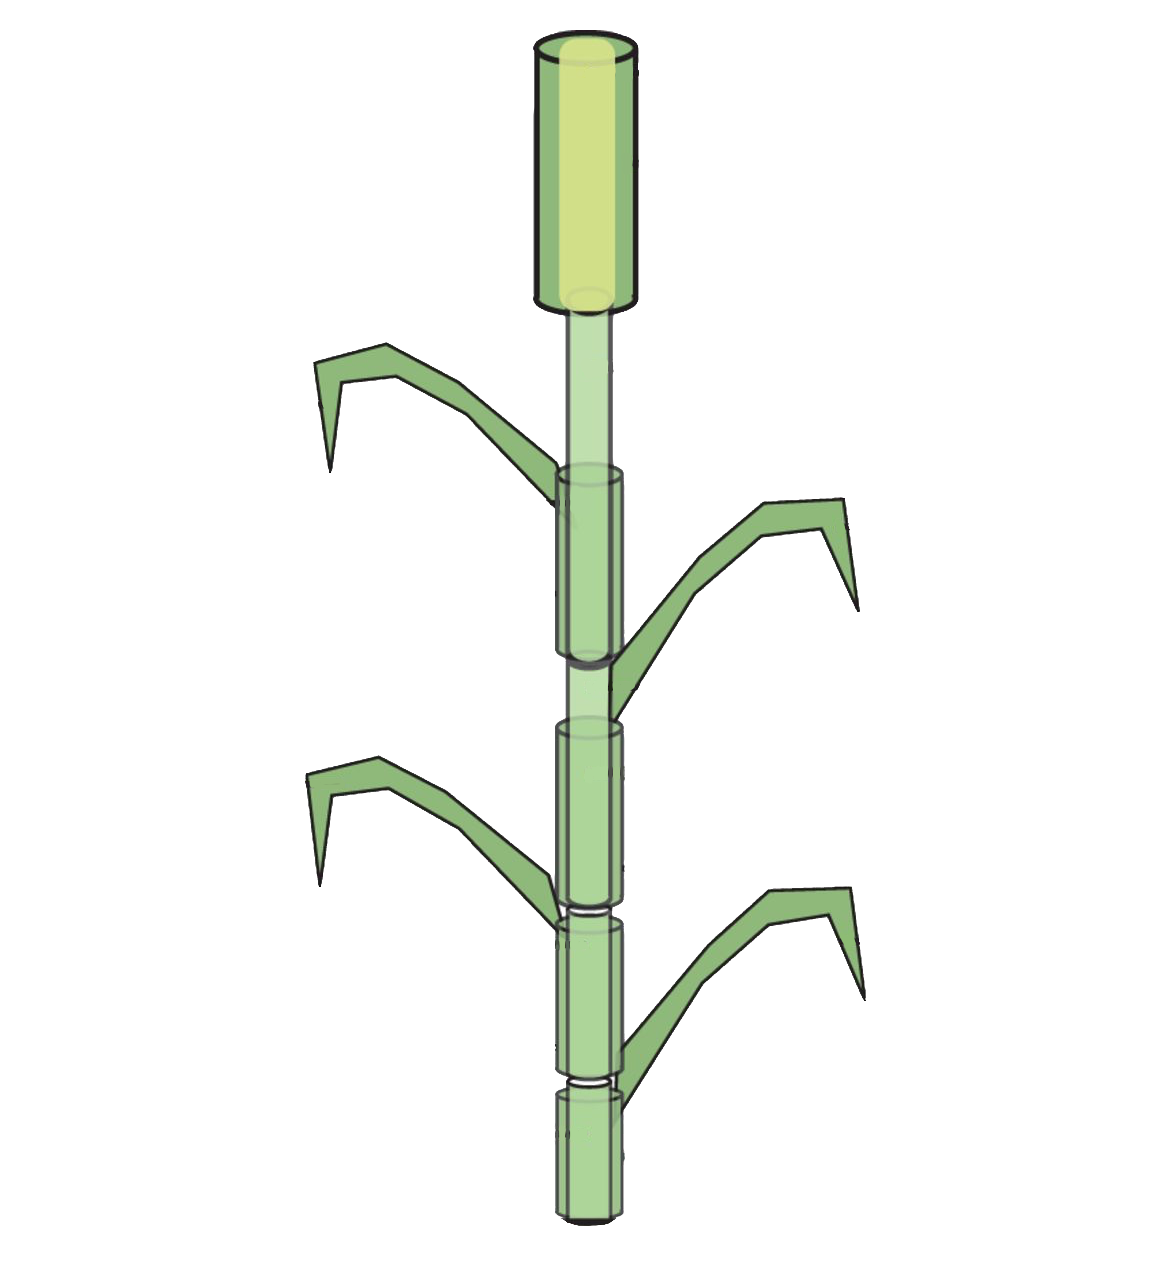
\includegraphics[width=0.2\textwidth]{figures/cnwheat} & 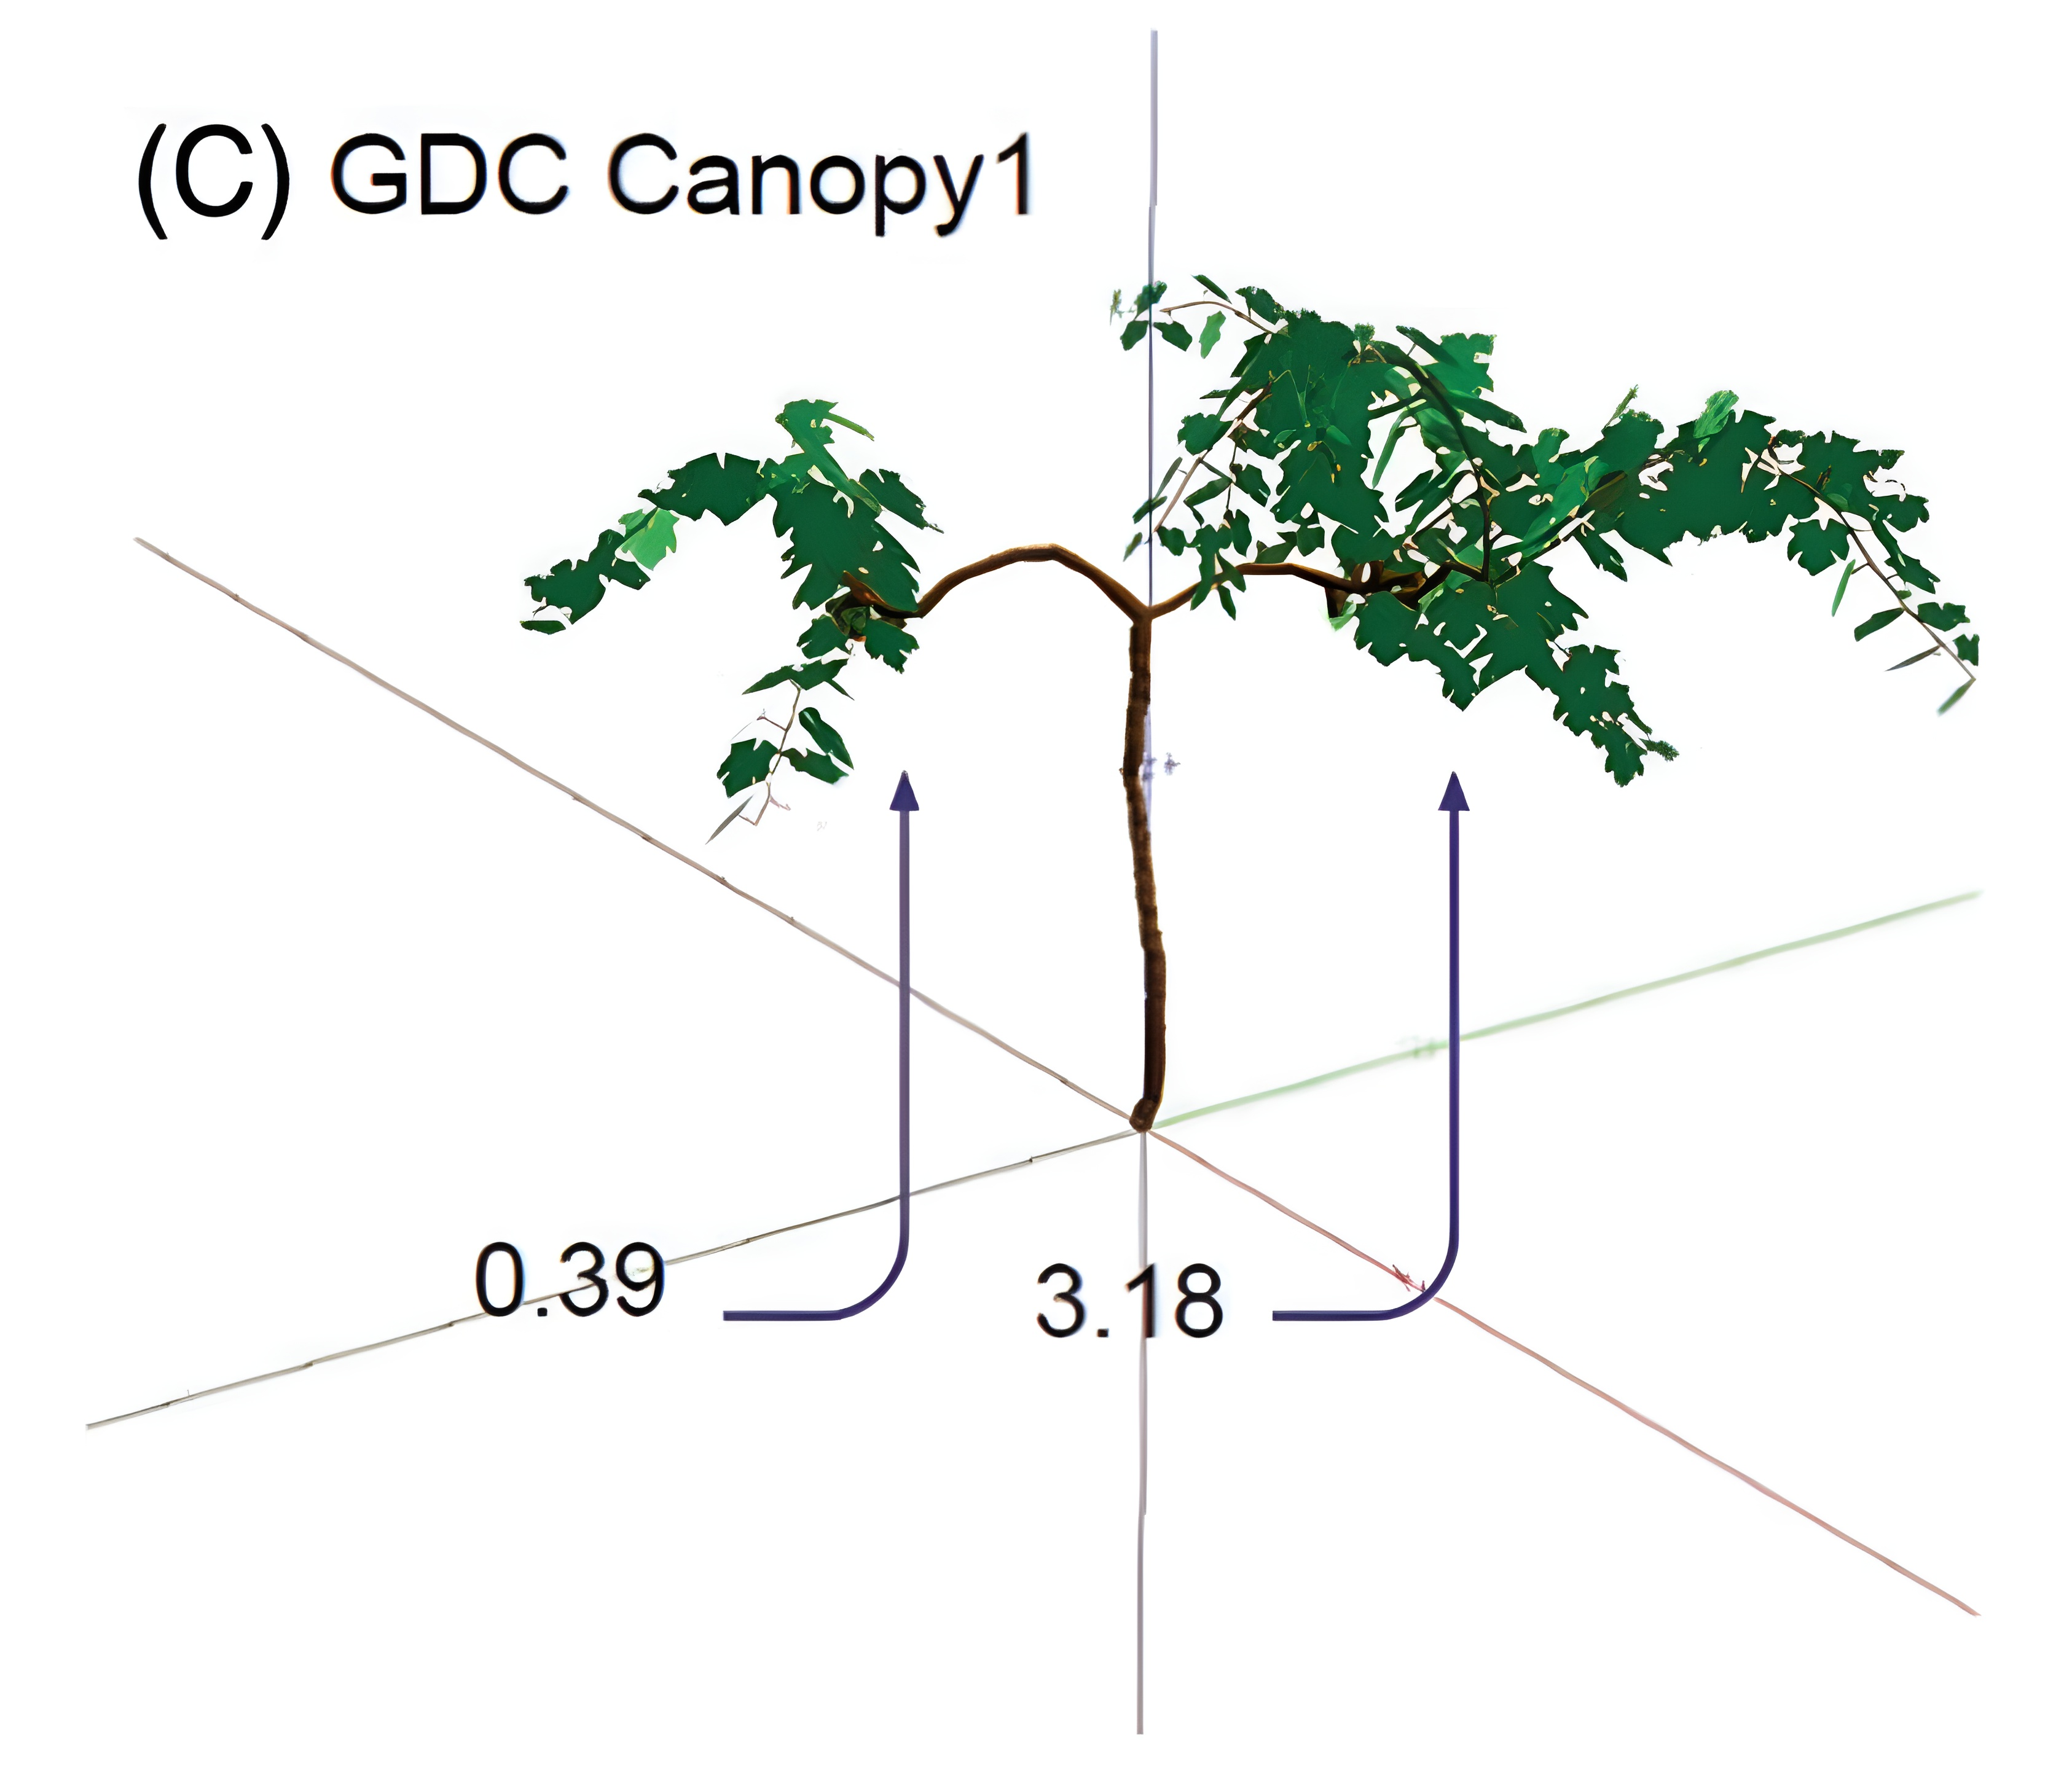
\includegraphics[width=0.2\textwidth]{figures/hydroshoot} & 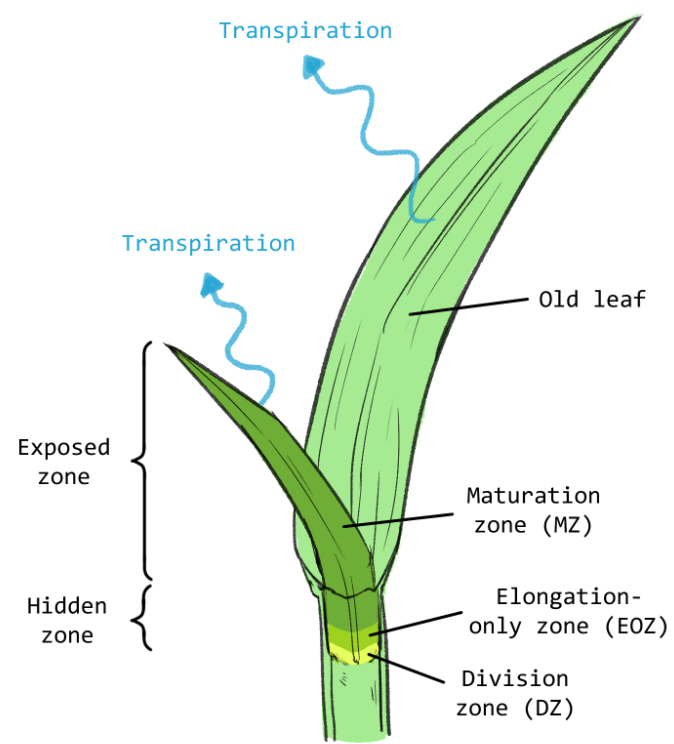
\includegraphics[width=0.2\textwidth]{figures/GrassLeaf} \\
 & \textbf{CN-Wheat} & \textbf{Hydroshoot} & \textbf{GrassLeaf} \\
 & {\footnotesize (Barillot et al., 2016)} & {\footnotesize (Albasha et al., 2019)} & {\footnotesize (unpublished)} \\
\textbf{simulation step} & 1h & 1h & 1h \\
\textbf{simulation duration} & 7d + repeats & 50d & TODO \\
\textbf{model structure} & static & post-veg. growth & single organ \\
\textbf{model size} & approx. $10^3$ & 15 & TODO \\
\end{tabular}

\end{frame}

\begin{frame}{Overview of the Methodology (Practical Point of View)}

\centering

\begin{columns}
\begin{column}{0.47\linewidth}
\centering
\begin{tikzpicture}[every node/.style={draw,rounded corners,align=center}]
\node[] (run) {run the FSPM};
\node[below=0.5cm of run] (data) {collect output data\\into table by unit};
\node[below=0.5cm of data] (prep) {data preprocessing};
\node[below=0.5cm of prep] (train) {train Ridge regression};
\node[below=0.5cm of train] (eval) {evaluate on unseen data};

\draw[line>] (run) -- (data);
\draw[line>] (data) -- (prep);
\draw[line>] (prep) -- (train);
\draw[line>] (train) -- (eval);
\draw[line>] (prep.west) -- ++(-1,0) |- (eval);
\end{tikzpicture}
\end{column}%
\hfill%
\begin{column}{0.47\linewidth}
\centering
\begin{tikzpicture}
    \begin{axis}[
    	width=\linewidth,
    	height=\linewidth,
    	date coordinates in=x,
    	xticklabel={\month-\day},
    	xlabel={time},
    	ylabel={air temperature [\si{\degreeCelsius}]},
    	xtick={2012-06-01,2012-06-05,2012-06-09,2012-06-13},
    	]
        \addplot[line width=1pt] table[x=date, y=Tac, col sep=comma] {meteo.csv};
        
        \scoped[on background layer] \fill [blue3!50] (axis cs:2012-06-01 00:00,\noexpand\pgfkeysvalueof{/pgfplots/ymin}) rectangle (axis cs:2012-06-05 00:00,\noexpand\pgfkeysvalueof{/pgfplots/ymax});
        
        \scoped[on background layer] \fill [green2!50] (axis cs:2012-06-05 00:00,\noexpand\pgfkeysvalueof{/pgfplots/ymin}) rectangle (axis cs:2012-06-09 00:00,\noexpand\pgfkeysvalueof{/pgfplots/ymax});
        
        \scoped[on background layer] \fill [blue3!50] (axis cs:2012-06-09 00:00,\noexpand\pgfkeysvalueof{/pgfplots/ymin}) rectangle (axis cs:2012-06-13 00:00,\noexpand\pgfkeysvalueof{/pgfplots/ymax});
        
        \scoped[on background layer] \fill [green2!50] (axis cs:2012-06-13 00:00,\noexpand\pgfkeysvalueof{/pgfplots/ymin}) rectangle (axis cs:2012-06-14 00:00,\noexpand\pgfkeysvalueof{/pgfplots/ymax});
    \end{axis}
\end{tikzpicture}
\end{column}
\end{columns}
\end{frame}

\begin{frame}{Transpiration-based Reservoirs for Input Condition Prediction}

\centering

There should be an image here like in the paper

\end{frame}

\begin{frame}{Code and Results}

\url{https://doi.org/10.5281/zenodo.7701995}

Based on the master dissertation by UGent student Maxime Cannoodt.

\textbf{Olivier Pieters}
Maxime Cannoodt
Tom De Swaef
Michiel Stock
Francis wyffels
	
\end{frame}

\end{document}
